\section{Проектирование системы}
\label{sec:system-design}

\subsection{Обоснование архитектурного шаблона проектирования}
\label{sub:system-design:architectural-pattern-design}

На сетевом уровне, предполагающем рассмотрение взаимодействия различных систем через сеть, в основе разрабатываемой системы лежит архитектура «клиент-сервер», в которой задания или сетевая нагрузка распределены между поставщиками услуг (сервисов), называемых серверами, и заказчиками услуг, называемых клиентами. В качестве среды взаимодействия клиента с сервером используется сеть Интернет. На рис.~\ref{fig:client-server-architecture} показана диаграмма, отражающая взаимосвязь компонентов клиент-серверной архитектуры.

\begin{figure}[h]
\centering
    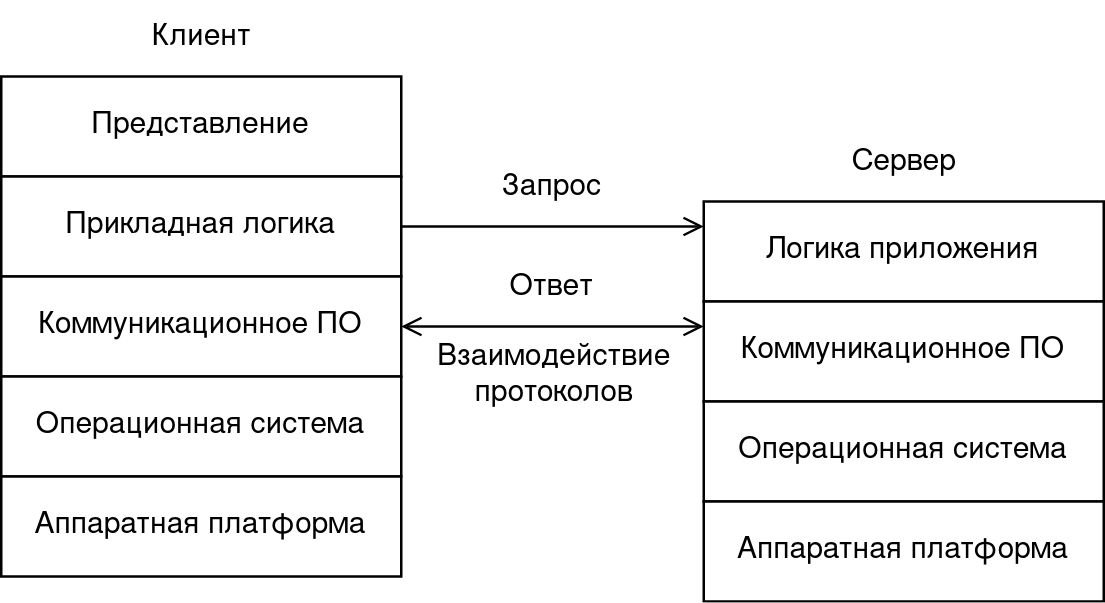
\includegraphics[width=0.75\linewidth]{assets/client-server-architecture.png}
    \caption{Схема архитектуры «клиент-сервер»}
    \label{fig:client-server-architecture}
\end{figure}

Основными достоинствами архитектуры «клиент-сервер» являются:

\begin{itemize}
    \item возможность, в большинстве случаев, распределить функции вычислительной системы между несколькими независимыми компьютерами в сети, что позволяет упростить обслуживание вычислительной системы, в частности, замена, ремонт, модернизация или перемещение сервера, не затрагивают клиентов;
    \item обеспечение хранения данных только на сервере, который, как правило, защищён гораздо лучше большинства клиентов, что позволит обеспечить контроль полномочий, чтобы разрешать доступ к данным только клиентам с соответствующими правами доступа;
    \item возможность объединения клиентов с разными аппаратными платформами, операционными системами для использования ресурсов одного сервера.
\end{itemize}

К основным недостаткам клиент-серверной архитектуры можно отнести:

\begin{itemize}
    \item неработоспособность основного сервера, в случае использования централизованной системы, может сделать неработоспособным всё приложение;
    \item потребность в наличии квалифицированного профессионала для администрирования системы;
    \item высокая стоимость оборудования.
\end{itemize}

В ходе выбора аппаратной платформы в данном дипломном проекте будут предложены и реализованы решения, позволяющие минимизировать вероятность выхода из строя серверной части приложения, а также позволяющие снизить стоимость оборудования до оплаты минимально необходимого уровня производительности.

Реализация серверной части системы, содержащей бизнес-логику и программный код, выполнена в соответствии с микросервисной архитектурой, которая представляет собой стиль разработки программного обеспечения, при котором система строится как набор небольших, автономных сервисов, каждый из которых отвечает за конкретный функциональный блок или бизнес-операцию. Единицей модульности является сервис. Сервис~-- это автономный, независимо развертываемый программный компонент, который реализует определенные полезные функции~\cite{book_microservices_patterns}. Схема микросервисной архитектуры представлена на рис.~\ref{fig:system-design:architectural-pattern-design:microservice-architecture}. В качестве коннекторов служат коммуникационные протоколы, которые позволяют сервисам взаимодействовать между собой.

\begin{figure}[h]
\centering
    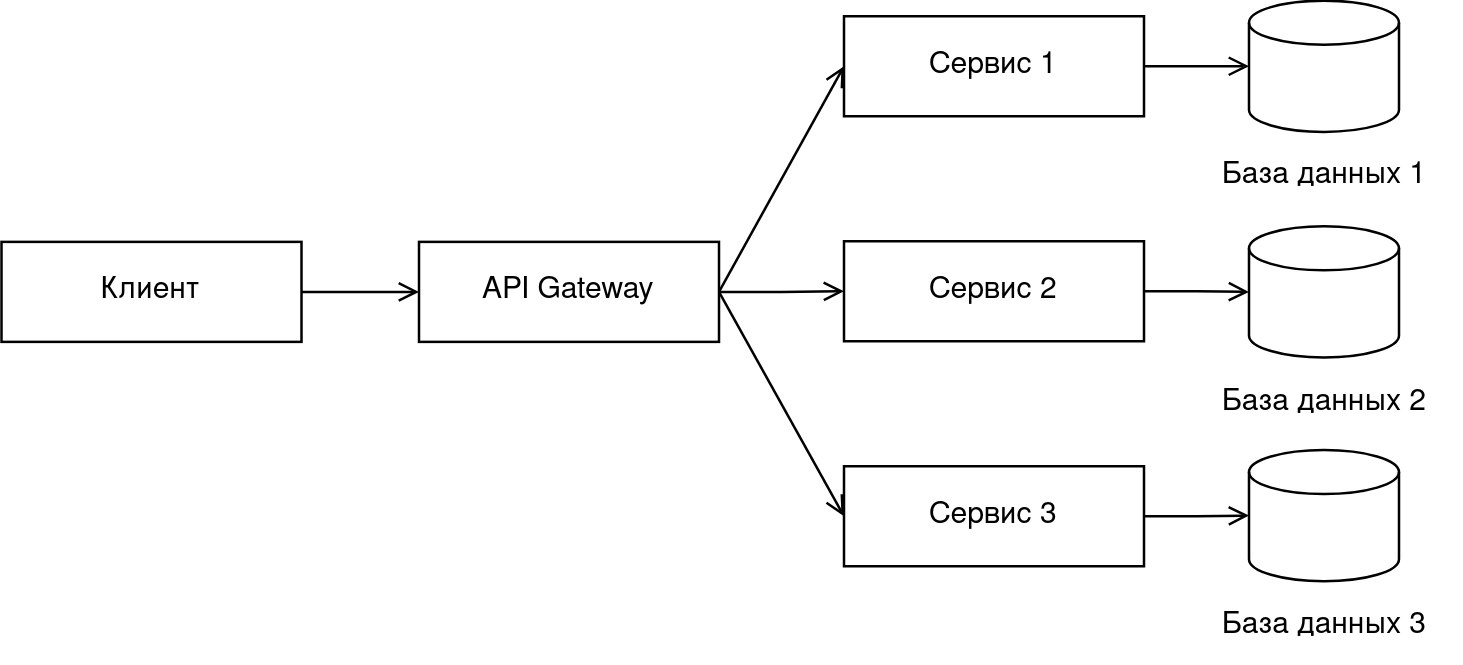
\includegraphics[width=0.9\linewidth]{assets/microservice-architecture.png}
    \caption{Схема микросервисной архитектуры}
    \label{fig:system-design:architectural-pattern-design:microservice-architecture}
\end{figure}

Основной стратегией создания микросервисной архитектуры является разбиение по бизнес-возможностям (поддоменам в предметно-ориен\-ти\-ро\-ван\-ном программировании). На рис.~\ref{fig:microservices-service-illustration} показано внешнее представление сервиса (в данном случае \textit{OfficeManagement}). Сервис обладает \textit{API}, который инкапсулирует реализацию. \textit{API} определяет операции, вызываемые клиентами. Существует два типа операций: команды (обновляют данные) и запросы (извлекают данные). При изменении своих данных сервис публикует события, на которые могут подписаться его клиенты. \textit{API} состоит из команд, запросов и событий. Команда, такая как \textit{\lstinline!create_workspace()!}, выполняет действия и обновляет данные. Запрос, такой как \textit{\lstinline!find_workspace()!}, извлекает данные. Сервис также публикует события, например
\textit{\lstinline!WorkspaceCreated!}, которые потребляются его клиентами. \textit{API} сервиса, который реализуется адаптерами, которые взаимодействуют с бизнес-логикой приложения, инкапсулирует его внутреннюю реализацию.

\begin{figure}[h]
\centering
    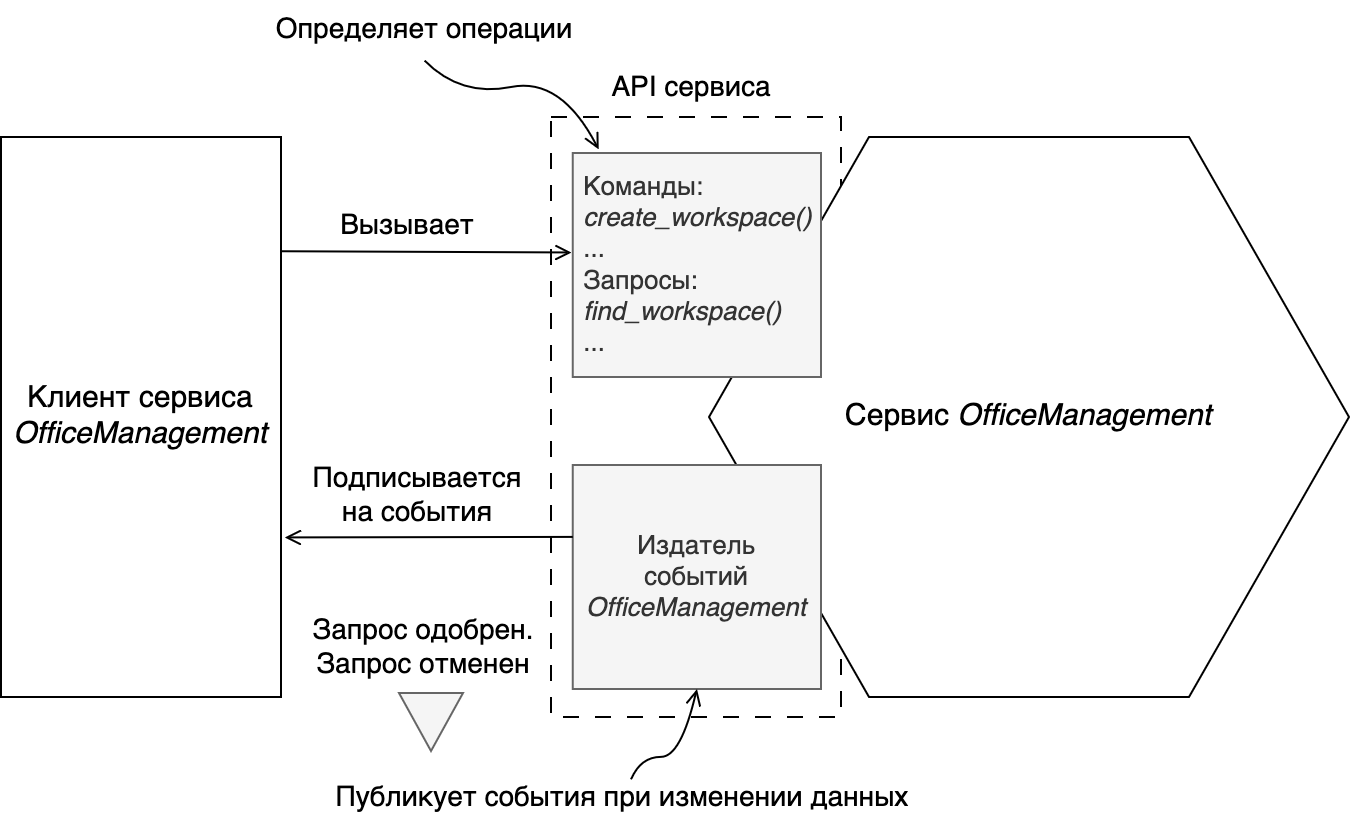
\includegraphics[width=0.9\linewidth]{assets/microservices-service-illustration.png}
    \caption{Внешнее представление сервиса \textit{OfficeManagement}}
    \label{fig:microservices-service-illustration}
\end{figure}

Достоинствами микросервисной архитектуры являются:

\begin{itemize}
    \item наличие возможности непрерывной доставки и независимого развертывания крупных, сложных приложений;
    \item сервисы получаются небольшими и простыми в обслуживании;
    \item позволяет экспериментировать и внедрять новые технологии;
    \item в ней лучше изолированы неполадки.
\end{itemize}

Возможность выполнять непрерывные доставку и развертывание обеспечивает несколько бизнес-преимуществ, например: компания обеспечивает уровень надежности своих услуг, соответствующий современным ожиданиям; работники довольны, поскольку вместо реализации сложных интеграций новых возможностей с существующей логикой они уделяют больше времени выпуску нового функционала.

Определение обязанностей каждого программного элемента является одной из основных задач проектирования программных продуктов. Принцип единственной ответственности \textit{SRP} гласит о том, что у класса должна быть только одна причина для изменения. Применяя \textit{SRP} к микросервисной архитектуре, получим совокупность небольших согласованных сервисов, обладающих одной обязанностью. Принцип согласованного изменения \textit{CCP} гласит о том, что причины изменения классов, входящих в один пакет, должны быть одинаковыми. Изменение пакета должно затрагивать все его классы. \textit{CCP} можно применить при создании микросервисной архитектуры, объединяя компоненты, изменяющиеся по одной и той же причине, в единый сервис, что позволит сократить количество сервисов, которые придется редактировать и заново развертывать при изменении какого-либо бизнес-требования.

Все сервисы и их \textit{API} имеют четкие определения. Каждый из них можно разрабатывать, тестировать, развертывать и масштабировать независимо от остальных. Такая архитектура помогает поддерживать модульность. Разработчик не может обратиться к внутренним компонентам сервиса, минуя его \textit{API}.

Важным шагом в определении архитектуры приложения является описание \textit{API} для каждого сервиса. Это реализуется путем назначения сервисам всех системных операций, определенных в перечне функциональных требований. Операция может быть реализована в виде одного или нескольких сервисов. В последнем случае необходимо решить, как они будут взаимодействовать между собой, что обычно требует поддержки дополнительных операций с их стороны. Также необходимо выбрать один из механизмов \textit{IPC}, чтобы реализовать \textit{API} каждого из сервисов.

После описания обобщенной доменной модели необходимо определить перечень запросов, которые приложение должно обрабатывать. В реализуемой системе большинство запросов основаны на \textit{HTTP}, однако вполне вероятно, что некоторым клиентам необходим механизм обмена сообщениями. Таким образом, вместо привязки к конкретному протоколу для представления запросов лучше использовать более абстрактное понятие системной операции~\cite{book_microservices_patterns}.

Системные операции бывают двух типов:
\begin{itemize}
    \item \textit{команды}~-- системные операции для создания, обновления и удаления данных;
    \item \textit{запросы}~-- системные операции для чтения (запрашивания) данных.
\end{itemize}

Бизнес-логика реализуемой системы состоит из нескольких бэкенд-сервисов. У каждого из них есть \textit{REST API} и собственная приватная база данных. Схема соответствия между бизнес-возможностями и сервисами разрабатываемой системы показана на рис.~\ref{fig:system-design:architectural-pattern-design:microservices-business-use-case}. Сервисам соответствуют возможности разных уровней иерархии.

\begin{figure}
\centering
    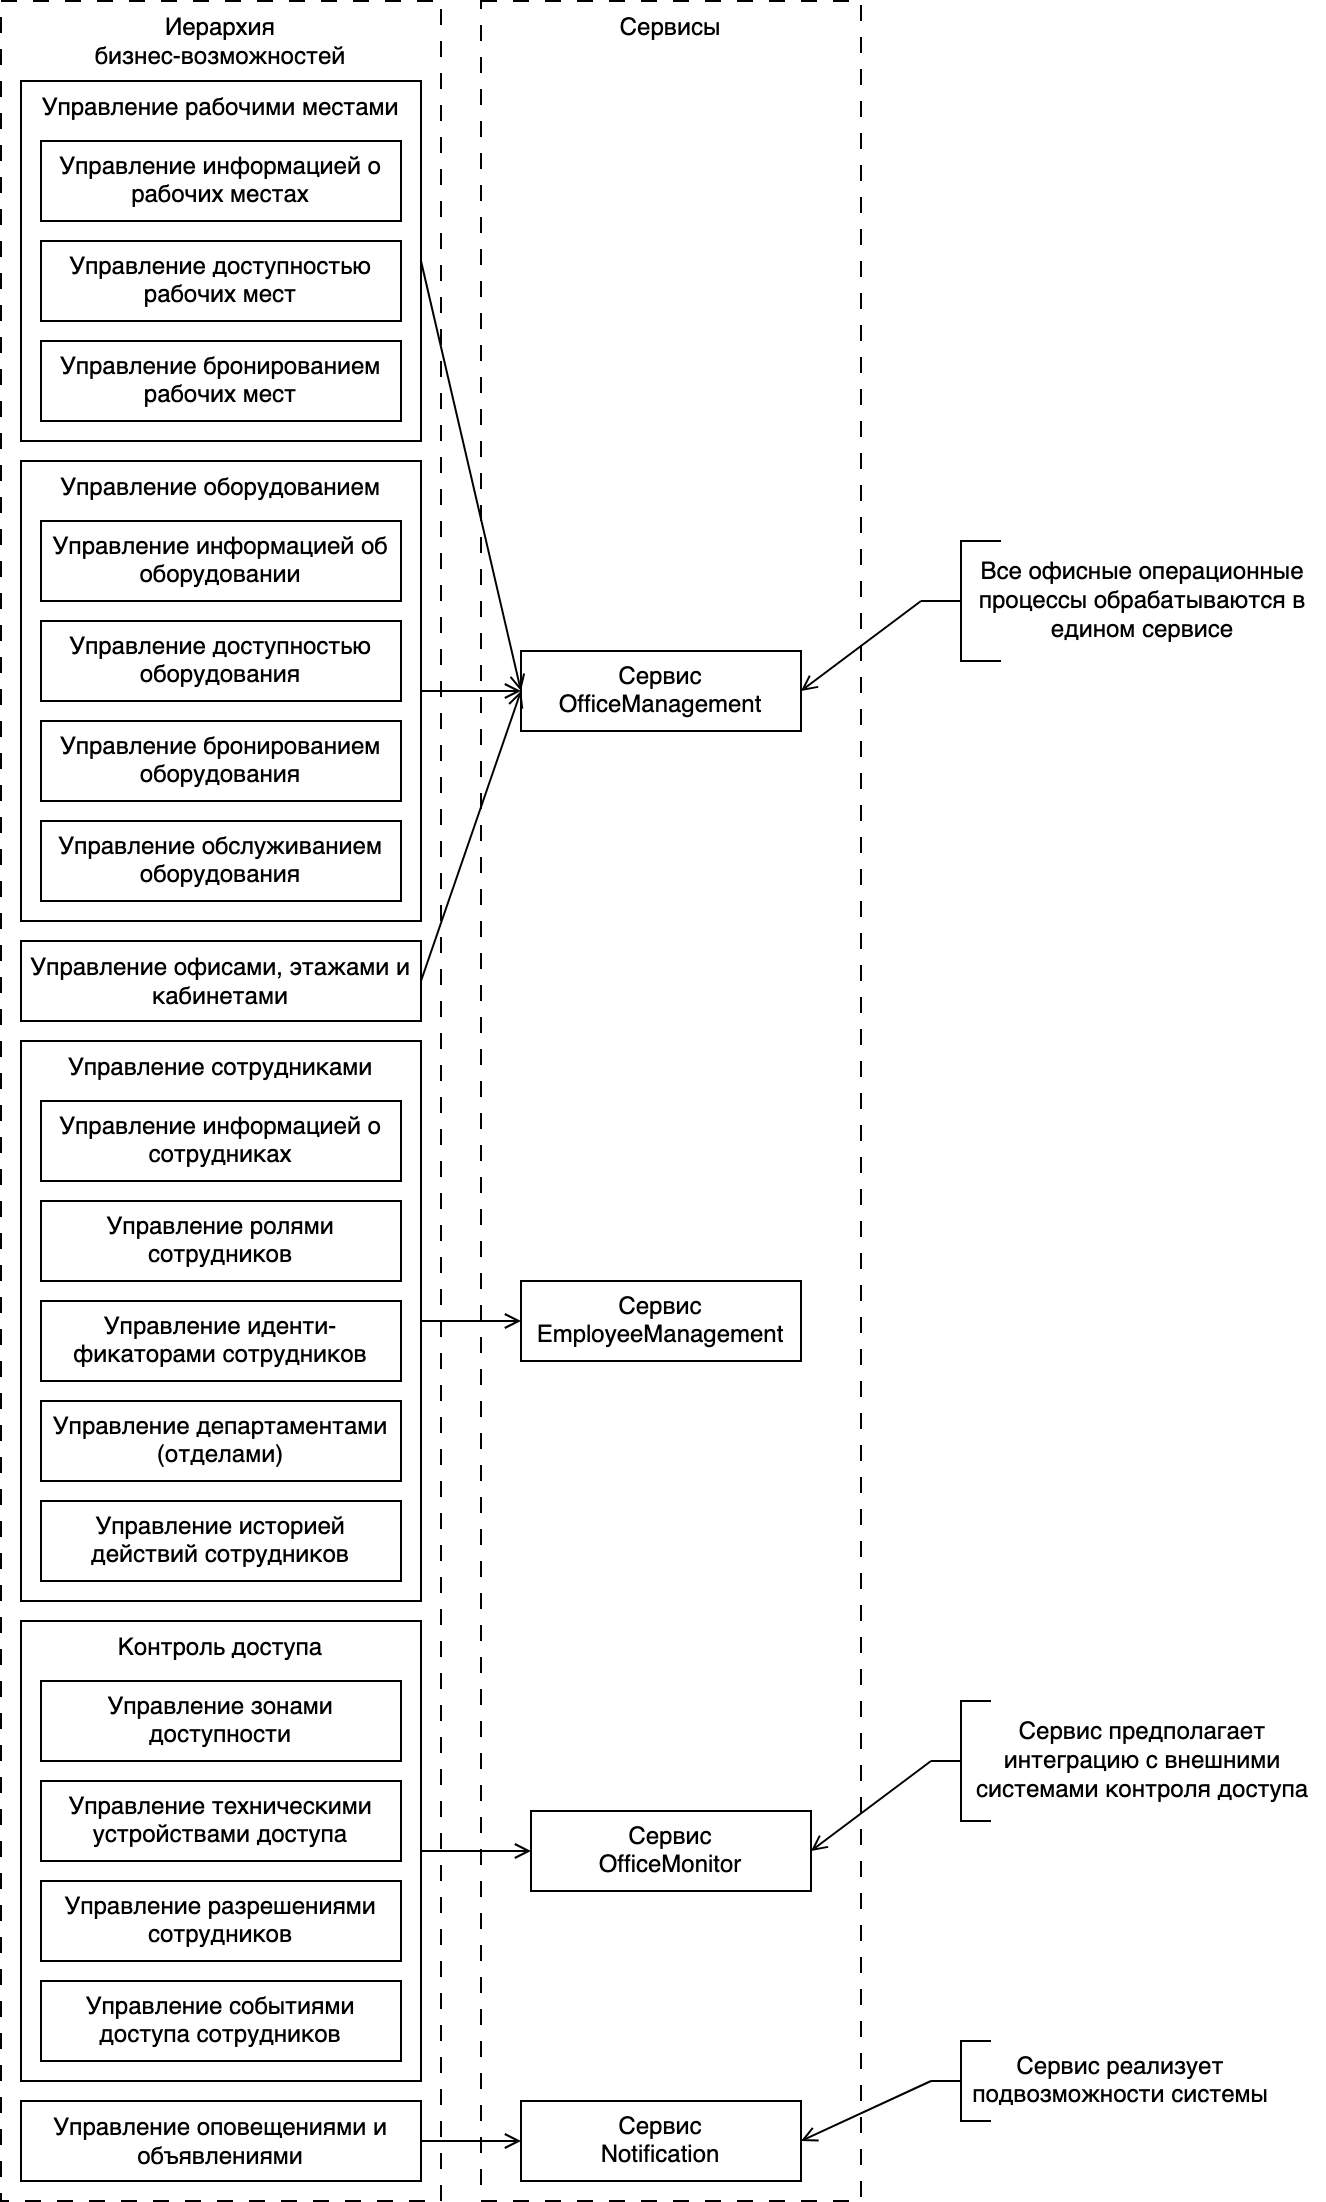
\includegraphics[width=0.8\linewidth]{assets/microservices-business-use-cases.png}
    \caption{Схема соответствия бизнес-возможностей и сервисов разрабатываемой системы}
    \label{fig:system-design:architectural-pattern-design:microservices-business-use-case}
\end{figure}

Сервисами системы являются:

\label{page:system-design:architectural-pattern-design:microservices-list}
\begin{itemize}
    \item \textit{EmployeeManagement} - управляет сотрудниками;
    \item \textit{OfficeManagement} - управляет операционными процессами;
    \item \textit{OfficeMonitor} - управляет контролем доступа и посещаемости;
    \item \textit{Notification} - отвечает за отправку уведомлений пользователям системы.
\end{itemize}

Иногда сервисы создаются для возможностей верхнего уровня, таких как управление рабочими местами или контроль доступа, а иногда~-- для подвозможностей, например, управление оповещениями и объявлениями.

Сервисы могут взаимодействовать через \textit{API}: примитивные каналы, такие как брокеры сообщений или простые протоколы, подобные \textit{REST} или \textit{gRPC}. Асинхронный \textit{API} состоит из операций, вызываемых клиентами, и событий, которые публикуют сервисы. В реализуемой системе используется подход с использованием асинхронного обмена сообщениями, что имеет неоспоримое преимущество~-- отсутствие блокировки клиента в ожидании ответа с расчетом на то, что ответ может прийти не сразу. Как видно на рис.~\ref{fig:microservices-broker-messaging}, сообщения передаются по каналам. Бизнес-логика отправителя обращается к интерфейсу исходящего порта, который реализуется адаптером отправителя сообщения. Отправитель шлет сообщение получателю через канал. Канал сообщений~-- это абстракция инфраструктуры обмена сообщениями. Адаптер обработчика сообщений в получателе вызывается для обработки сообщения. Он обращается к интерфейсу входящего порта, который реализуется бизнес-логикой получателя.

\begin{figure}[h]
\centering
    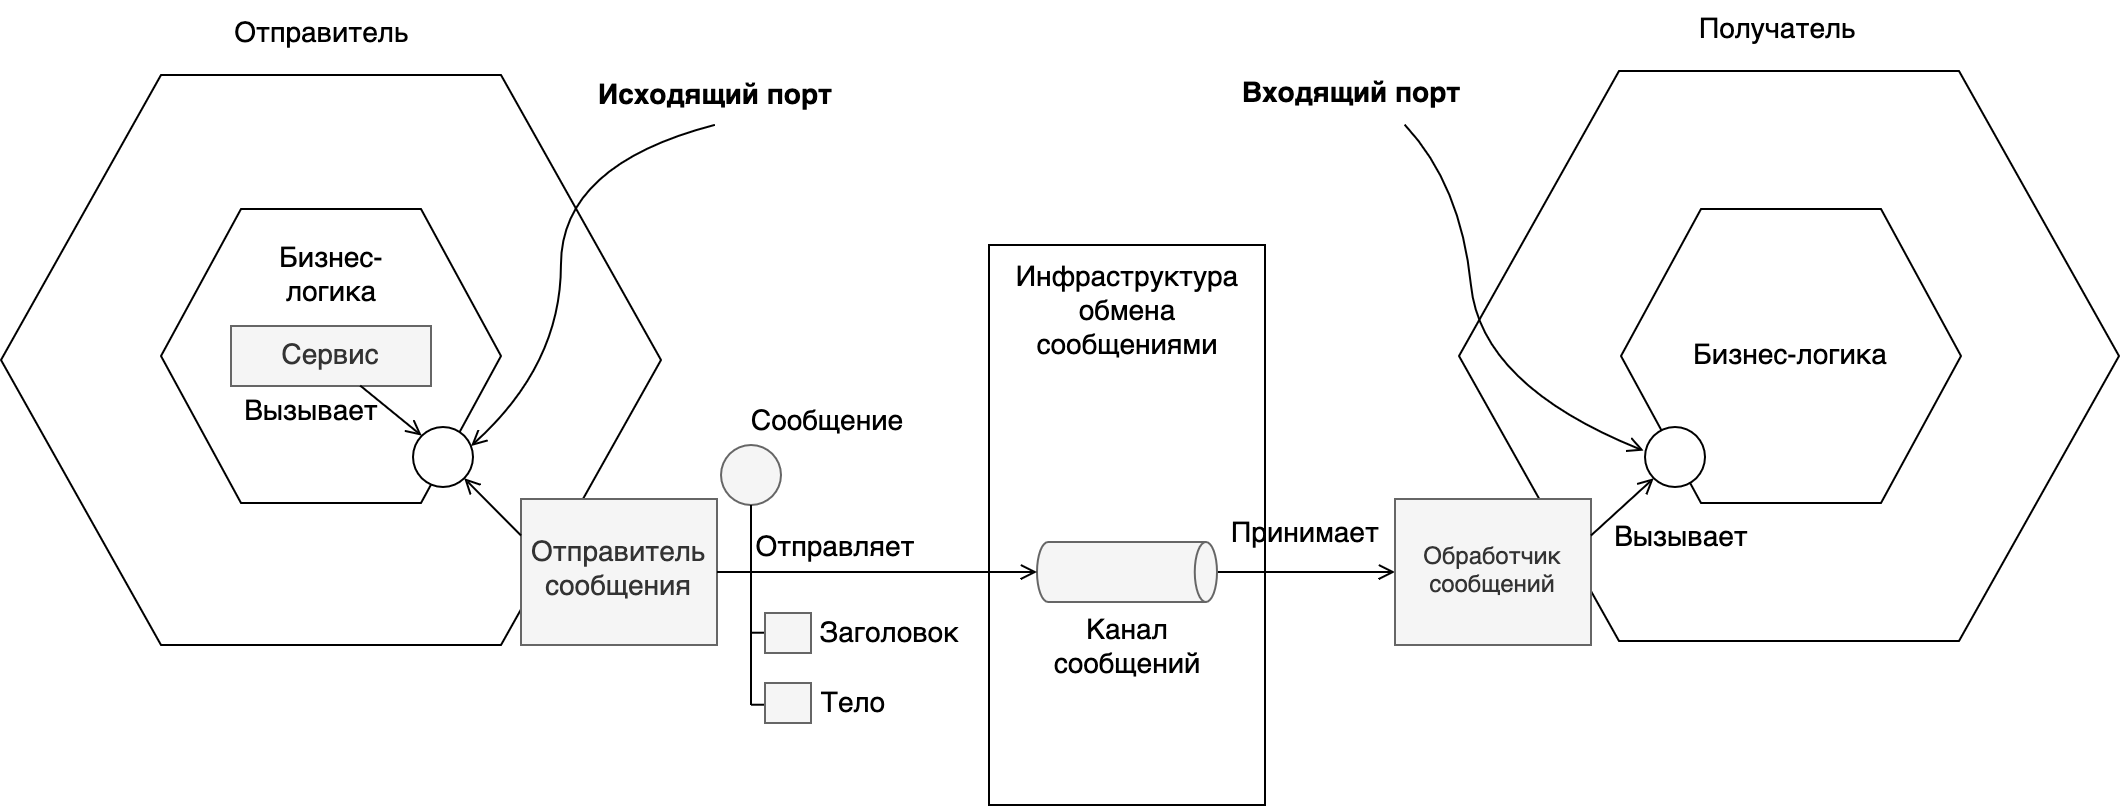
\includegraphics[width=1\linewidth]{assets/microservices-broker-messaging.png}
    \caption{Структура процесса передачи сообщений, используя брокер сообщений}
    \label{fig:microservices-broker-messaging}
\end{figure}

Архитектурный стиль \textit{REST} (\textit{Representational State Transfer}) \textit{API}~-- это стиль для разработки веб-сервисов, который основывается на принципах и ограничениях, способствующих созданию распределённых систем. В контексте веб-программирования, \textit{REST API} представляет собой набор интерфейсов, через которые клиентские приложения могут взаимодействовать с сервером с помощью стандартных \textit{HTTP}-методов, таких как \textit{GET}, \textit{POST}, \textit{PUT}, \textit{DELETE}. Эти методы используются для получения, отправки, обновления или удаления данных. \textit{RESTful}-сервисы обеспечивают лёгкость интеграции и взаимодействия между компонентами системы, поскольку они используют стандартные протоколы передачи данных (например, \textit{JSON} или \textit{XML}).

В \textit{REST} определяется строгое разделение ответственности между компонентами клиент-серверной системы, облегчающее реализацию необходимых актеров (\textit{actors}). Другой целью \textit{REST} является упрощение семантики взаимодействия компонентов сетевых систем, что позволяет улучшить масштабируемость и повысить производительность. В основу \textit{REST} заложен принцип автономности запросов, означающий, что запросы, обрабатываемые клиентом или сервером, должны включать всю контекстную информацию, необходимую для их понимания. При работе \textit{REST}-систем для обмена данными стандартных медиа-типов используется минимальное количество запросов. \textit{REST}-системы используют \textit{URI} (универсальные идентификаторы ресурсов) для поиска и получения доступа к представлениям необходимых ресурсов.

Клиент должен сообщить сервису, куда тому следует вернуть результат, и сопоставить ответное сообщение со своим запросом. Для этого клиент отправляет командное сообщение с каналом ответа в заголовке. Сервер записывает в этот канал свой ответ, содержащий идентификатор соответствия с тем же значением, что и идентификатор запроса. Клиент использует идентификатор соответствия, чтобы сопоставить свое сообщение с ответом.

Как результат, микросервисная архитектура стала неотъемлемой частью любой компании, зависящей от программных технологий.


\subsection{Обоснование выбора инструментальных средств разработки}
\label{sub:system-design:dev-tools}

В этом разделе будет произведено рассмотрение основных технологий, использованных при разработке системы.

Для реализации \textit{backend}-архитектуры системы используются следующие технологии:

\begin{itemize}
    \item язык программирования \textit{Python};
    \item веб-фреймворк \textit{FastAPI};
    \item \textit{SQLAlchemy}, \textit{Alembic}, \textit{Pydantic} для взаимодействия с базой данных, выполнения миграций и реализации \textit{ORM}~-- технологии программирования, которая связывает базы данных с концепциями объектно-ориентированных языков программирования, создавая «виртуальную объектную базу данных».
\end{itemize}

Выбор \textit{Python} обусловлен его активным развитием, популярностью в сфере веб-разработки и удобством для работы с асинхронными операциями. \textit{SQLAlchemy} обеспечивает удобное взаимодействие с реляционными базами данных, сокращая количество \textit{SQL}-запросов и повышая читаемость кода.

Реализация клиентской части системы выполнена с использованием следующих технологий:

\begin{itemize}
    \item языков программирования \textit{JavaScript}, \textit{TypeScript};
    \item языков разметки и стилистического оформления \textit{HTML} и \textit{CSS};
    \item библиотеки \textit{React} для разработки пользовательских интерфейсов;
    \item CSS-фреймворков \textit{Tailwind}, \textit{MaterialUI}.
\end{itemize}

Выбор \textit{React} обусловлен наличием компонентного подхода, упрощающего поддержку и масштабируемость кода. \textit{Tailwind CSS} ускоряет верстку за счет готовых классов, а \textit{MaterialUI} предоставляет набор компонентов для обеспечивания удобного и современного пользовательского интерфейса.

В качестве СУБД используется \textit{PostgreSQL} из-за её бесплатного распространения, высокой производительности, надёжности, поддержкой \textit{ACID}-транзакций и расширяемости.

Для развёртывания системы на сервере используется совокупность технологий:

\begin{itemize}
    \item \textit{Docker} для контейнеризации приложений;
    \item \textit{Kubernetes(k3s)} для оркестрации приложений, обеспечивая автоматическое управление нагрузкой, балансировку трафика, восстановление контейнеров в случае сбоя;
\end{itemize}

Системой контроля версий является \textit{Git}, выбранный веб-сервис для хостинга проекта~-- \textit{GitHub}. Технологией непрерывной интеграции/непрерывного развертывания является \textit{GitHub Actions}.


% -------------------------- Убрано
\iffalse

\subsubsection{Язык программирования Python. }

Python~-- это высокоуровневый язык программирования общего назначения. Он является интерпретируемым, то есть его код исполняется непосредственно интерпретатором без предварительной компиляции в машинный код, что позволяет достичь кроссплатформенности, поэтому приложения на Python могут запускаться на различных операционных системах (Windows, macOS, Linux и др.) без необходимости модификации исходного кода. При этом Python автоматически компилирует исходный код в промежуточный байт-код (файлы с расширением .pyc), который затем исполняется интерпретатором. Наиболее популярная реализация Python~-- CPython, написанная на языке C. CPython предоставляет интерпретатор, стандартную библиотеку и возможности для интеграции с модулями на C для повышения производительности.

В программировании активно используются фреймворки~-- структуры, которые предоставляют разработчику готовые инструменты, библиотеки и архитектурные решения для упрощения создания приложений. В экосистеме Python представлено множество фреймворков, охватывающих широкий спектр задач. Например, для веб-разработки существуют Django, Flask, FastAPI и Pyramid, для машинного обучения~-- TensorFlow, PyTorch и Scikit-learn, для тестирования~-- pytest и unittest, а для создания графических интерфейсов~-- PyQt, Tkinter и Kivy.

Веб-фреймворки Python предназначены для упрощения разработки веб-приложений, предоставляя необходимый инструментарий для реализации серверной логики, маршрутизации запросов, работы с базами данных и аутентификации пользователей. FastAPI~-- современный фреймворк, оптимизированный для создания высокопроизводительных API с использованием стандартов OpenAPI и JSON Schema.

Таким образом, Python, благодаря своей интерпретируемости, динамической типизации и богатой экосистеме, является одним из самых популярных языков программирования, а разнообразие фреймворков делает его подходящим для решения практически любых задач в разработке.

\subsubsection{СУБД PostgreSQL. }

PostgreSQL~-- это мощная реляционная система управления базами данных (СУБД) с открытым исходным кодом, которая отличается высокой производительностью, надёжностью и расширяемостью. Она соответствует стандарту SQL:2016 и поддерживает такие продвинутые возможности, как оконные функции, Common Table Expressions (CTE) и полнотекстовый поиск. PostgreSQL обеспечивает выполнение ACID-транзакций, гарантируя целостность данных даже в критических ситуациях, и поддерживает сложные типы данных, включая JSON/JSONB, массивы, XML и пользовательские структуры.

Одним из ключевых преимуществ PostgreSQL является её расширяемость. Разработчики могут создавать собственные типы данных, функции, операторы и индексы, а также использовать множество сторонних расширений, таких как PostGIS для работы с геоданными или TimescaleDB для временных рядов. Система эффективно работает с аналитическими и транзакционными нагрузками, обеспечивая параллельное выполнение запросов, масштабируемость и поддержку репликации (как синхронной, так и асинхронной). Для оптимизации запросов PostgreSQL предоставляет широкий выбор индексов, включая B-Tree, GiST, GIN, BRIN и другие, что делает её универсальной для различных сценариев использования.

По сравнению с другими реляционными СУБД, PostgreSQL обладает рядом преимуществ. Во-первых, это мощная поддержка JSONB, которая позволяет использовать её как гибридную базу данных для работы с документами, конкурируя с NoSQL-системами, такими как MongoDB. Во-вторых, PostgreSQL отличается высокой универсальностью: она одинаково эффективна для транзакционных систем (OLTP) и аналитических систем (OLAP), благодаря поддержке сложных запросов и массивов. В-третьих, система легко масштабируется и поддерживает высокую доступность с помощью таких инструментов, как Patroni и Pgpool-II. Кроме того, благодаря поддержке Foreign Data Wrappers (FDW), PostgreSQL может интегрироваться с другими базами данных и внешними источниками данных~\cite{book_postgres_optimization}.

Особое внимание заслуживает продвинутая система индексации. PostgreSQL позволяет использовать уникальные индексы, такие как GiST и GIN, что делает её идеальной для работы с полнотекстовым поиском и пространственными данными. Благодаря открытому исходному коду PostgreSQL активно развивается и получает регулярные обновления, а её большое сообщество обеспечивает доступ к обширной документации и решениям для специфических задач.

PostgreSQL широко применяется для создания веб-приложений, построения аналитических систем, работы с геоданными и JSON-документами, а также в сценариях, требующих высокой производительности и надёжности. Благодаря своей гибкости, функциональности и поддержке масштабирования, PostgreSQL является одним из лидеров среди современных реляционных СУБД, сочетая в себе возможности классических баз данных и гибкость NoSQL-систем.

\subsubsection{Язык программирования TypeScript и фреймворк React. }

TypeScript и React~-- это современные инструменты, которые часто используются для разработки масштабируемых, производительных и поддерживаемых веб-приложений.

TypeScript представляет собой надмножество JavaScript, добавляющее статическую типизацию и расширенные возможности для разработки, такие как поддержка интерфейсов, перегрузка функций и объединение типов. Код TypeScript компилируется в стандартный JavaScript, что делает его совместимым с любой платформой или браузером. Одним из ключевых преимуществ TypeScript является статическая типизация, которая позволяет выявлять ошибки уже на этапе компиляции.

React~-- это библиотека для построения пользовательских интерфейсов, разработанная Facebook. Она предлагает декларативный стиль программирования, позволяя разработчику описывать, как интерфейс должен выглядеть в зависимости от состояния приложения. Её ключевое преимущество~-- компонентный подход, который позволяет разбивать интерфейс на независимые, многократно используемые компоненты. React использует виртуальный DOM для эффективного обновления только изменённых компонентов вместо полной перерисовки всей страницы~\cite{book_react}.

Таким образом, использование TypeScript в сочетании с React позволяет разработчикам строить современные веб-приложения, которые отличаются высокой надёжностью, эффективностью и удобством поддержки. TypeScript обеспечивает строгую типизацию и улучшенный контроль кода, а React предлагает гибкость и мощные инструменты для создания интерфейсов, делая их сочетание особенно привлекательным для сложных и долгосрочных проектов.

\subsubsection{Технологии развёртывания. }

Docker и Kubernetes~-- это ключевые технологии современной разработки, которые обеспечивают контейнеризацию и оркестрацию приложений. Они играют важную роль в упрощении развертывания, управления и масштабирования программных решений.

Контейнеризация представляет собой метод упаковки приложений и всех их зависимостей в изолированные среды, называемые контейнерами. Эти контейнеры используют общее ядро операционной системы, что делает их лёгкими, производительными и удобными для переноса между различными средами. Основные преимущества контейнеризации включают портативность (контейнеры работают одинаково на любых платформах), эффективное использование ресурсов (благодаря отсутствию необходимости эмулировать полноценную ОС, как в виртуальных машинах), изоляцию приложений для повышения безопасности, а также упрощение разработки и развертывания за счёт стандартизированных сред.

Docker~-- это платформа, предназначенная для создания, развертывания и управления контейнерами. С его помощью разработчики могут создавать образы контейнеров с использованием Dockerfile, управлять ими через Docker Registry, а также запускать контейнеры с минимальными накладными расходами. Docker предоставляет возможности для работы с сетями, хранения данных и автоматизации жизненного цикла контейнеров.

Однако для управления множеством контейнеров в масштабах кластера Docker нуждается в системе оркестрации, что достигается с помощью Kubernetes. Kubernetes~-- это открытая система оркестрации, которая автоматизирует развертывание, управление и масштабирование контейнеризированных приложений. Она изначально была разработана Google и предоставляет богатый функционал для управления контейнерными кластерами.

Одним из ключевых преимуществ Kubernetes является автоматическое масштабирование и репликация приложений. С помощью механизма ReplicaSet система гарантирует, что всегда будет поддерживаться заданное количество копий контейнеров, что обеспечивает надёжность и устойчивость к сбоям. Kubernetes также упрощает сетевое взаимодействие: компонент Ingress позволяет маршрутизировать входящие запросы к контейнерам через HTTP/HTTPS, настраивать балансировку нагрузки и SSL-шифрование. Кроме того, поддержка сетевых политик позволяет разработчикам контролировать, как трафик проходит между компонентами приложения.

Управление состоянием приложений в Kubernetes реализовано через Persistent Volume (PV) и Persistent Volume Claim (PVC), которые обеспечивают удобное хранение данных, даже если контейнеры перезапускаются~\cite{book_production_kubernetes}. Система поддерживает обновления приложений без простоев (rolling updates) и откаты на предыдущие версии, если в процессе развертывания возникают проблемы. Kubernetes также обеспечивает высокую доступность приложений благодаря встроенным механизмам отказоустойчивости, включая мониторинг состояния контейнеров через Liveness и Readiness Probes.

Ещё одно значимое преимущество Kubernetes~-- это его расширяемость. Пользовательские ресурсы (Custom Resource Definitions, CRD) позволяют добавлять новые типы объектов, а богатая экосистема включает инструменты для мониторинга (Prometheus), журналирования (ELK), автоматизации CI/CD (ArgoCD) и многое другое. Kubernetes также предоставляет встроенные механизмы для управления конфигурациями (ConfigMaps) и секретами (Secrets), что упрощает хранение и использование конфиденциальных данных.

Вместе Docker и Kubernetes создают мощную платформу для разработки, развертывания и эксплуатации современных приложений. Docker упрощает процесс контейнеризации, а Kubernetes обеспечивает эффективное управление этими контейнерами на уровне кластера, предоставляя инструменты для репликации, отказоустойчивости, маршрутизации через Ingress и управления состоянием. Эти технологии формируют основу облачной инфраструктуры, поддерживая автоматизацию, масштабируемость и высокую доступность приложений.

\subsubsection{Технологии непрерывной интеграции/непрерывного развертывания. }

CI/CD (Continuous Integration/Continuous Deployment)~-- это подход и набор инструментов, направленных на автоматизацию ключевых этапов разработки программного обеспечения, включая тестирование, сборку и развертывание. Эти методы помогают ускорить процесс разработки, повысить качество кода и уменьшить вероятность ошибок, делая проект более стабильным и готовым к частым обновлениям.

Continuous Integration (CI) подразумевает регулярное объединение изменений в коде с основной веткой репозитория. Каждый коммит или запрос на слияние запускает автоматизированный процесс проверки, включающий тестирование и сборку приложения. Цель CI~-- выявлять ошибки на ранних стадиях разработки, предотвращая проблемы, которые могут возникнуть при интеграции изменений.

Continuous Deployment (CD) автоматизирует процесс доставки изменений в различные среды~-- тестовую, промежуточную или к конечным пользователям. В рамках подхода Continuous Delivery развертывание требует подтверждения человека, в то время как в Continuous Deployment все изменения, успешно прошедшие тесты, автоматически развёртываются. Это сокращает время выхода обновлений и минимизирует человеческий фактор.

При разработке данной системы использовался GitHub Actions - инструмент для автоматизации CI/CD, встроенный в экосистему GitHub. Он предоставляет возможность автоматического запуска процессов в ответ на события в репозитории, такие как внесение изменений, создание запросов на слияние или выпуск новой версии.

\fi
% -------------------------- Убрано


\subsection{Проектирование и реализация моделей базы данных}
\label{sub:system-design:database-model}

Реляционные системы управления базами данных являются стандартным подходом при проектировании веб-приложений, поскольку удовлетворяют следующим критериям:

\begin{itemize}
    \item поддержание полноты и целостности хранимых данных за счет механизмов уникальности данных, внешних и первичных ключей, наложения ограничений на данные и контроля их связности;
    \item поддержка свойства транзакционности, позволяющее выполнять нес\-коль\-ко операций как неделимое действие и возвращать данные в прошлое состояние в случае провала фиксации данных;
    \item поддержка требований \textit{ACID}: \textit{Atomicity} (атомарность), \textit{Consistency} (согласованность), \textit{Isolation} (изоляция) и \textit{Durability} (долговечность), которые обеспечивают надежность обработки данных.
\end{itemize}

В реализуемой системе структура базы данных представляет собой комплексное решение для управления офисными помещениями, информацией о сотрудниках, контролем доступа и посещаемости, и распределением рабочих мест. 

Как было упомянуто в разделе~\ref{sub:system-design:architectural-pattern-design} на странице~\pageref{page:system-design:architectural-pattern-design:microservices-list}, используемый подход микросервисной архитектуры предполагает наличие нескольких приватных баз данных для каждого сервиса, что обеспечивает изоляцию данных и независимость компонентов. Такой подход позволяет каждому сервису самостоятельно управлять своей схемой данных и выбирать наиболее подходящую технологию хранения, соответствующую специфике бизнес-логики. Разделение данных способствует более четкому разграничению ответственности между командами разработки, а также усиливает инкапсуляцию, предотвращая нежелательные зависимости на уровне базы данных. Кроме того, отказ от общей базы данных позволяет избежать узких мест, связанных с централизованным управлением транзакциями, и минимизировать влияние изменений схемы данных одного сервиса на другие. Такой подход был выбран для обеспечения гибкости системы в условиях высокой нагрузки, а также для упрощения сопровождения и эволюции сервисов в рамках распределенной архитектуры.

Логическая модель базы данных представляется в виде \textit{ER}-модели данных, которая предназначена для описания объектов и отношений базы данных. Основными понятиями модели \textit{ER} являются: сущность (\textit{entity})~-- объект, который идентифицируется человеком конкретно в предметной области; атрибуты~-- значимые характеристики сущности; связи~-- отношения между различными сущностями. На рис.~\ref{fig:system-design:database-model:erd} представлена схема базы данных.

\afterpage{
    \clearpage
    \begin{landscape}
        \thispagestyle{landscape}
        \begin{figure}[p]
            \centering
            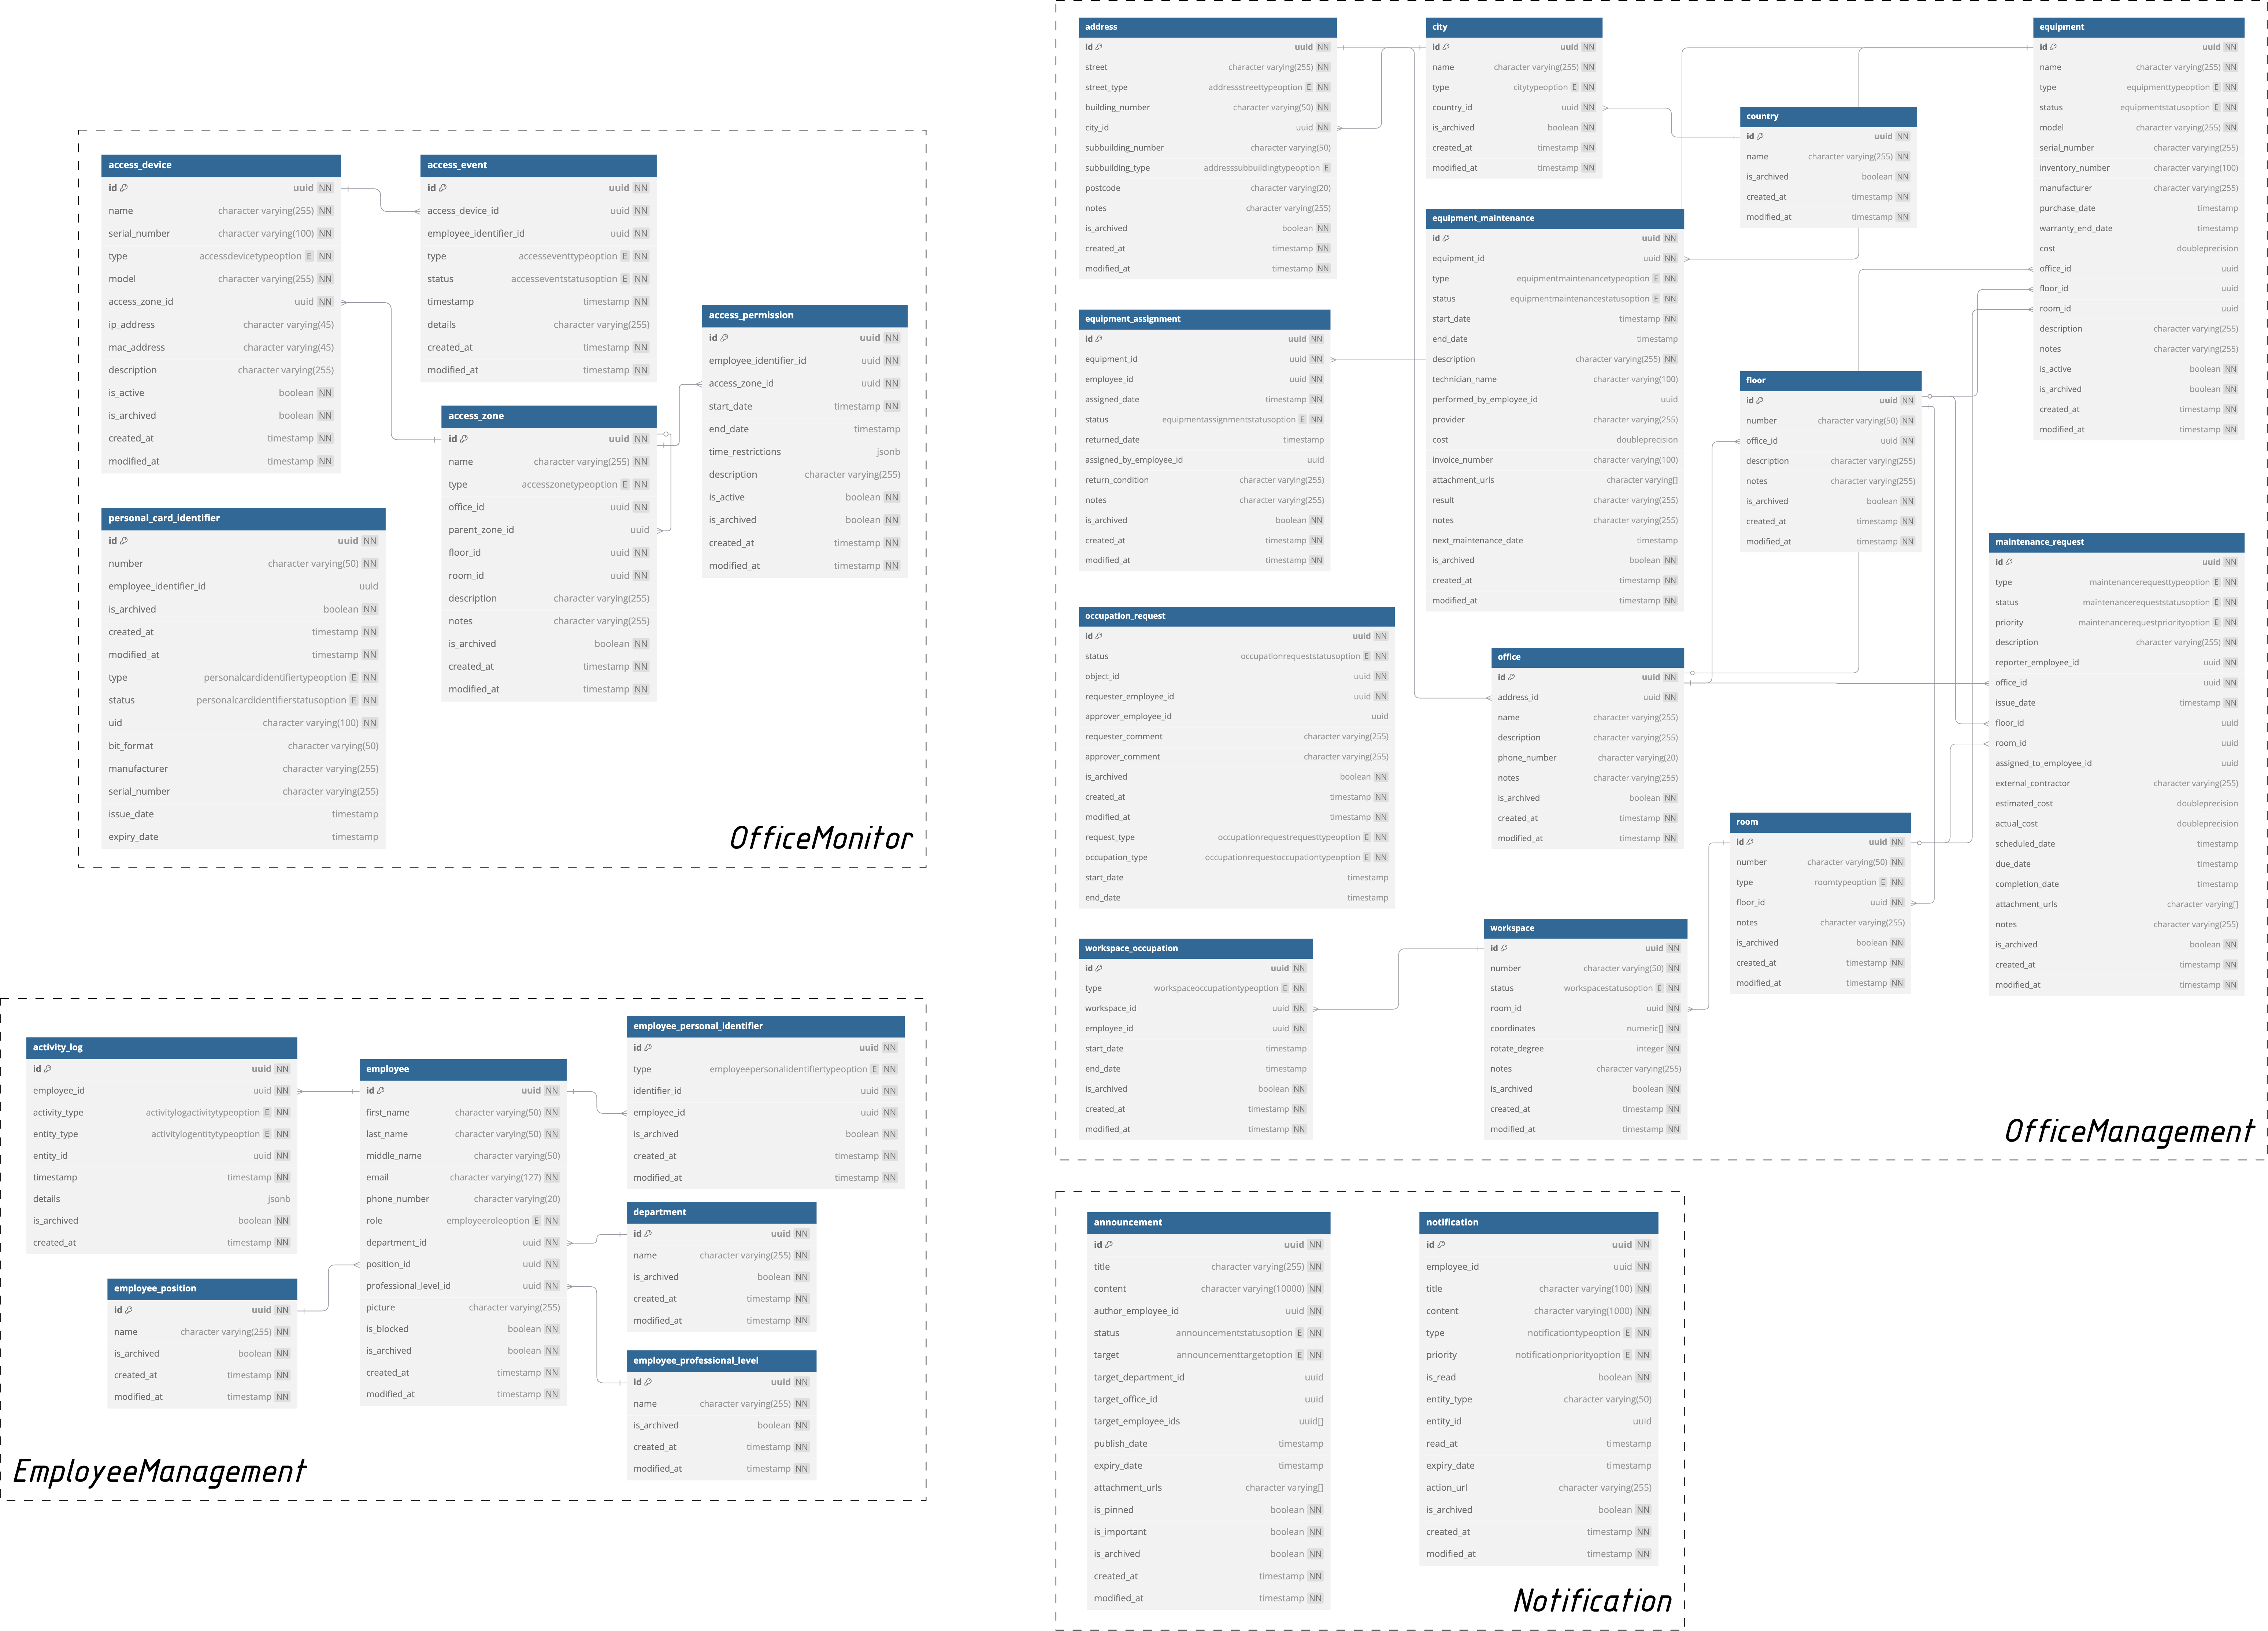
\includegraphics[width=0.8\linewidth]{assets/ERD.png}
            \caption{Схема базы данных}
            \label{fig:system-design:database-model:erd}
        \end{figure}
    \end{landscape}
    \clearpage
}

Рассмотрим структуру базы данных сервиса \textbf{\textit{EmployeeManagement}}, реализующего бизнес-логику операций управления сотрудниками, авторизации и аутентификации в системе. Записи о сотрудниках включают контактную информацию, положение в организации, набор прав и привилегий, и профессиональные атрибуты.

Организационная структура: Отдел → Сотрудник → Должность/профессиональный уровень. Система управления сотрудниками фиксирует отношения подчинения, пути профессионального развития и организацию отдела. Это позволяет выполнять такие \textit{HR}-функции, как составление организационных схем и отслеживание карьерного роста. В таблицах~\ref{table:system-design:database-model:employee-schema},~\ref{table:system-design:database-model:activity_log-schema} представлено подробное описание типов для таблиц «Сотрудник», «Действие» базы данных сервиса \textit{EmployeeManagement}.

Сотрудник занимает определённую должность и имеет установленный профессиональный уровень, а также принадлежит к отделу. Каждому сотруднику соответствует уникальная запись с контактной информацией и ролью в компании. Все действия сотрудников фиксируются в журнале активности, где указывается тип действия, над какой сущностью оно выполнено и дополнительные детали. В таблице «Действие» хранится ссылка на сотрудника, совершившего действие, через внешний ключ. Таким образом, можно отследить, какие действия выполнял конкретный сотрудник. Связи между таблицами обеспечиваются внешними ключами с ограничением на удаление \textit{RESTRICT}, что предотвращает потерю важной информации. Эти взаимосвязи позволяют контролировать активность персонала, а также структурировать и анализировать поведение сотрудников по должности, отделу и уровню.

\begingroup
\singlespacing
\vspace{-\baselineskip}
\begin{longtable}{| >{\raggedright}m{0.29\textwidth} 
                  | >{\raggedright}m{0.35\textwidth} 
                  | >{\raggedright}m{0.15\textwidth} 
                  | >{\raggedright\arraybackslash}m{0.1\textwidth}|}
    \caption{Типы данных сущности «Сотрудник»} \label{table:system-design:database-model:employee-schema} \\ \hline
    Атрибут & Название & Тип & Размер \\ \hline
    \endfirsthead
    \multicolumn{4}{@{}l}{\noindent Продолжение таблицы~\thetable} \\ \hline
    Атрибут & Название & Тип & Размер \\ \hline
    \endhead
    \textit{id} & Идентификатор & \textit{UUID} & - \\ \hline
    \textit{first\_name} & Имя & Строка & 50 \\ \hline
    \textit{last\_name} & Фамилия & Строка & 50 \\ \hline
    \textit{middle\_name} & Отчество & Строка & 50 \\ \hline
    \textit{email} & Адрес электронной почты & Строка & 127 \\ \hline
    \textit{phone\_number} & Номер телефона & Строка & 20 \\ \hline
    \textit{role} & Роль сотрудника & Строка & 15 \\ \hline
    \textit{department\_id} & Внешний ключ на столбец \textit{ID} в таблице «Отдел» & \textit{UUID} & - \\ \hline
    \textit{position\_id} & Внешний ключ на столбец \textit{ID} в таблице «Должность» & \textit{UUID} & - \\ \hline
    \textit{professional\_level\_id} & Внешний ключ на столбец \textit{ID} в таблице «Профессиональный уровень» & \textit{UUID} & - \\ \hline
    \textit{picture} & Путь к изображению (ссылка) & Строка & 255 \\ \hline
    \textit{is\_blocked} & Флаг блокировки сотрудника & Булево & - \\ \hline
    \textit{is\_archived} & Флаг архивирования записи сотрудника & Булево & - \\ \hline
    \textit{created\_at} & Временная метка создания записи & Дата и время & - \\ \hline
    \textit{modified\_at} & Временная метка изменения записи & Дата и время & - \\ \hline
\end{longtable}
\endgroup

\begingroup
\singlespacing
\vspace{-\baselineskip}
\begin{longtable}{| >{\raggedright}m{0.29\textwidth} 
                  | >{\raggedright}m{0.35\textwidth} 
                  | >{\raggedright}m{0.15\textwidth} 
                  | >{\raggedright\arraybackslash}m{0.1\textwidth}|}
    \caption{Типы данных сущности «Действие»} \label{table:system-design:database-model:activity_log-schema} \\ \hline
    Атрибут & Название & Тип & Размер \\ \hline
    \endfirsthead
    \multicolumn{4}{@{}l}{\noindent Продолжение таблицы~\thetable} \\ \hline
    Атрибут & Название & Тип & Размер \\ \hline
    \endhead
    \textit{id} & Идентификатор & \textit{UUID} & - \\ \hline
    \textit{employee\_id} & Внешний ключ на столбец \textit{ID} в таблице «Сотрудник» & \textit{UUID} & - \\ \hline
    \textit{activity\_type} & Тип действия & Строка & 31 \\ \hline
    \textit{entity\_type} & Тип сущности, над которой было совершено действие & Строка & 31 \\ \hline
    \textit{entity\_id} & Внешний ключ на столбец \textit{ID} в таблице к сущности, над чем было совершено действие & \textit{UUID} & - \\ \hline
    \textit{timestamp} & Временная метка совершения действия & Дата и время & - \\ \hline
    \textit{details} & Дополнительные детали действия & \textit{JSONB} & - \\ \hline
    \textit{is\_archived} & Флаг архивирования записи & Булево & - \\ \hline
    \textit{created\_at} & Временная метка создания записи & Дата и время & - \\ \hline
\end{longtable}
\endgroup


Структура базы данных сервиса \textbf{\textit{OfficeManagement}}, предназначенного для осуществления управления офисными операционными процессами, построена на нескольких взаимосвязанных доменах.

Географическая и физическая иерархия пространства: Страна → Город → Адрес → Офис → Этаж → Помещение → Рабочее место. Такая иерархическая структура позволяет точно управлять местоположением нескольких офисов, которые могут находиться в разных странах. Такая структура поддерживает организации с международным присутствием, сохраняя при этом детализированный контроль вплоть до отдельных рабочих мест.

Управление рабочими местами: Рабочее место → Запрос на бронирование → Занятость рабочего места. В системе реализовано гибкое распределение рабочих мест с помощью записей о занятости мест, поддерживающих как постоянное, так и временное бронирование рабочих мест. Такая гибкость позволяет использовать такие современные методы работы, как гибридные форматы работы или наличие нескольких рабочих мест. В таблицах~\ref{table:system-design:database-model:workspace-schema},~\ref{table:system-design:database-model:workspace_occupation-schema},~\ref{table:system-design:database-model:room-schema} представлено подробное описание типов для таблиц «Рабочее место», «Бронирование рабочего места», «Кабинет» базы данных сервиса \textit{OfficeManagement}.

\begingroup
\singlespacing
\vspace{-\baselineskip}
\begin{longtable}{| >{\raggedright}m{0.29\textwidth} 
                  | >{\raggedright}m{0.35\textwidth} 
                  | >{\raggedright}m{0.15\textwidth} 
                  | >{\raggedright\arraybackslash}m{0.1\textwidth}|}
    \caption{Типы данных сущности «Рабочее место»} \label{table:system-design:database-model:workspace-schema} \\ \hline
    Атрибут & Название & Тип & Размер \\ \hline
    \endfirsthead
    \multicolumn{4}{@{}l}{\noindent Продолжение таблицы~\thetable} \\ \hline
    Атрибут & Название & Тип & Размер \\ \hline
    \endhead
    \textit{id} & Идентификатор & \textit{UUID} & - \\ \hline
    \textit{number} & Номер рабочего места & Числовой & - \\ \hline
    \textit{status} & Идентификатор & Строка & 15 \\ \hline
    \textit{room\_id} & Внешний ключ на столбец \textit{ID} в таблице «Кабинет» & \textit{UUID} & - \\ \hline
    \textit{coordinates} & Координаты положения рабочего места на плане этажа & Числовой (2) & - \\ \hline
    \textit{rotate\_degree} & Градус поворота & Числовой & - \\ \hline
    \textit{notes} & Дополнительные сведения, примечания & Строка & 255 \\ \hline
    \textit{is\_archived} & Флаг архивирования записи & Булево & - \\ \hline
    \textit{created\_at} & Временная метка создания записи & Дата и время & - \\ \hline
    \textit{modified\_at} & Временная метка изменения записи & Дата и время & - \\ \hline
\end{longtable}
\endgroup

Полный процесс создания и утверждения запросов на бронирование реализуется с помощью модели \textit{OccupationRequestModel} и соответствующей таблицы базы данных, хранящей записи о:

\begin{itemize}
    \item нескольких состояний статуса (в процессе, одобрен, отклонен, отложен, отменен);
    \item сотруднике, который создал запрос и сотруднике, утвердившим запрос;
    \item комментариях сотрудников;
\end{itemize}

\begingroup
\singlespacing
\vspace{-\baselineskip}
\begin{longtable}{| >{\raggedright}m{0.29\textwidth} 
                  | >{\raggedright}m{0.35\textwidth} 
                  | >{\raggedright}m{0.15\textwidth} 
                  | >{\raggedright\arraybackslash}m{0.1\textwidth}|}
    \caption{Типы данных сущности «Бронирование рабочего места»} \label{table:system-design:database-model:workspace_occupation-schema} \\ \hline
    Атрибут & Название & Тип & Размер \\ \hline
    \endfirsthead
    \multicolumn{4}{@{}l}{\noindent Продолжение таблицы~\thetable} \\ \hline
    Атрибут & Название & Тип & Размер \\ \hline
    \endhead
    \textit{id} & Идентификатор & \textit{UUID} & - \\ \hline
    \textit{type} & Тип бронирования (временное, постоянное) & Строка & 15 \\ \hline
    \textit{workspace\_id} & Внешний ключ на столбец \textit{ID} в таблице «Рабочее место» & \textit{UUID} & - \\ \hline
    \textit{employee\_id} & Внешний ключ на столбец \textit{ID} в таблице «Сотрудник» & \textit{UUID} & - \\ \hline
    \textit{start\_date} & Дата начала бронирования & Дата и время & - \\ \hline
    \textit{end\_date} & Дата окончания бронирования & Дата и время & - \\ \hline
    \textit{is\_archived} & Флаг архивирования записи & Булево & - \\ \hline
    \textit{created\_at} & Временная метка создания записи & Дата и время & - \\ \hline
    \textit{modified\_at} & Временная метка изменения записи & Дата и время & - \\ \hline
\end{longtable}
\endgroup

\begingroup
\singlespacing
\vspace{-\baselineskip}
\begin{longtable}{| >{\raggedright}m{0.29\textwidth} 
                  | >{\raggedright}m{0.35\textwidth} 
                  | >{\raggedright}m{0.15\textwidth} 
                  | >{\raggedright\arraybackslash}m{0.1\textwidth}|}
    \caption{Типы данных сущности «Кабинет»} \label{table:system-design:database-model:room-schema} \\ \hline
    Атрибут & Название & Тип & Размер \\ \hline
    \endfirsthead
    \multicolumn{4}{@{}l}{\noindent Продолжение таблицы~\thetable} \\ \hline
    Атрибут & Название & Тип & Размер \\ \hline
    \endhead
    \textit{id} & Идентификатор & \textit{UUID} & - \\ \hline
    \textit{number} & Номер кабинета & Строка & 7 \\ \hline
    \textit{type} & Тип кабинета & Строка & 31 \\ \hline
    \textit{floor\_id} & Внешний ключ на столбец \textit{ID} в таблице «Этаж» & \textit{UUID} & - \\ \hline
    \textit{notes} & Дополнительные сведения, примечания & Строка & 255 \\ \hline
    \textit{is\_archived} & Флаг архивирования записи & Булево & - \\ \hline
    \textit{created\_at} & Временная метка создания записи & Дата и время & - \\ \hline
    \textit{modified\_at} & Временная метка изменения записи & Дата и время & - \\ \hline
\end{longtable}
\endgroup


Сервис \textbf{\textit{OfficeMonitor}}, предназначенный для контроля доступа и посещаемости, предполагает наличие следующих доменных взаимоотношений.

Контроль доступа: Персональный идентификатор сотрудника → Идентификатор карты доступа. Процесс идентификации связывает сотрудников с учетными данными физического доступа, обеспечивая интеграцию с аппаратными устройствами безопасности.

Для всех таблиц используются различные методы, обеспечивающие надежную целостность данных. Последовательное использование первичных ключей \textit{UUID} обеспечивает глобальную уникальность для всех записей таблиц. Реализованы ограничения на внешние ключи с соответствующим поведением при удалении (\textit{RESTRICT}, \textit{CASCADE}, \textit{SET NULL})~\cite{book_postgres_optimization}. Все записи таблиц включают временные метки \textit{\lstinline!created_at!}  и \textit{\lstinline!modified_at!} для отслеживания изменений. Удаление с помощью флагов \textit{\lstinline!is_archived!} сохраняет исторические данные, позволяя при этом логически удалять их. Система использует типы перечислений для контролируемых словарей, включая: роли сотрудников \textit{EmployeeRoleOption}, типы комнат \textit{RoomTypeOption}, статусы рабочих мест \textit{WorkspaceStatusOption}, классификации городов \textit{CityTypeOption}, типы профессий \textit{WorkspaceOccupationTypeOption}.

В свою очередь, на программном уровне системы реализована всесторонняя проверка полей с помощью системы типов \textit{SQLAlchemy}.

Последовательное применение шаблонов проектирования во всех моделях обеспечивает удобство обслуживания, расширяемость и соответствие современным практикам работы с базами данных. Четкие взаимосвязи между сущностями создают целостную систему, способную эффективно моделировать сложную динамику современной офисной среды. В таблице~\ref{table:system-design:database-model:employee_personal_card_identifier-schema} представлено подробное описание типов для таблицы «Персональный идентификатор сотрудника~-- Карта» базы данных сервиса \textit{OfficeMonitor}.

\begingroup
\singlespacing
\vspace{-\baselineskip}
\begin{longtable}{| >{\raggedright}m{0.29\textwidth} 
                  | >{\raggedright}m{0.35\textwidth} 
                  | >{\raggedright}m{0.15\textwidth} 
                  | >{\raggedright\arraybackslash}m{0.1\textwidth}|}
    \caption{Типы данных сущности «Персональный идентификатор сотрудника~-- Карта»} \label{table:system-design:database-model:employee_personal_card_identifier-schema} \\ \hline
    Атрибут & Название & Тип & Размер \\ \hline
    \endfirsthead
    \multicolumn{4}{@{}l}{\noindent Продолжение таблицы~\thetable} \\ \hline
    Атрибут & Название & Тип & Размер \\ \hline
    \endhead
    \textit{id} & Идентификатор & \textit{UUID} & - \\ \hline
    \textit{number} & Номер карты & Строка & 50 \\ \hline
    \textit{type} & Тип карты & Строка & 15 \\ \hline
    status & Статус карты & Строка & 15 \\ \hline
    \textit{uid} & \textit{UID} & Строка & 100 \\ \hline
    \textit{employee\_identifier\_id} & Внешний ключ на столбец \textit{ID} в таблице «Персональный идентификатор сотрудника» & \textit{UUID} & - \\ \hline
    \textit{bit\_format} & \textit{Bit}-формат записи данных & Строка & 50 \\ \hline
    \textit{manufacturer} & Производитель & Строка & 255 \\ \hline
    \textit{serial\_number} & Серийный номер & Строка & 255 \\ \hline
    \textit{issue\_date} & Временная метка выпуска карты & Дата и время & - \\ \hline
    \textit{expiry\_date} & Временная метка истечения срока годности (эксплуатации) карты & Дата и время & - \\ \hline
    \textit{is\_archived} & Флаг архивирования записи & Булево & - \\ \hline
    \textit{created\_at} & Временная метка создания записи & Дата и время & - \\ \hline
\end{longtable}
\endgroup


\subsection{Алгоритмы работы системы}
\label{sub:system-design:algorithms}

В общем случае, алгоритм программы представляет собой весь цикл использования программного продукта, начиная с попадания пользователя на начальную страницу и заканчивая получением пользователем желаемых (отчетов, данных).

\textbf{\textit{Алгоритм утверждения запроса на бронирование рабочего места}} является одним из ключевых сценариев в системе управления офисными ресурсами является. Алгоритм реализует бизнес-логику, при которой менеджер, обладающий соответствующими правами, проверяет и одобряет или отклоняет поступивший от сотрудника запрос. После утверждения запроса система резервирует указанное рабочее место за сотрудником, обновляя его статус. Алгоритм проверки и утверждения бронирования содержит в себе несколько этапов проверки правильности входных значений и операций с базой данных.

\begin{enumerate}
    \item \textit{Получение запроса на бронирование}. Из базы данных извлекается объект запроса по его идентификатору. Если запрос помечен как архивный, то дальнейшая обработка запрещается и выполнение завершается с ошибкой. Если запрос помечен как уже обработанный, то выполнение также завершается с ошибкой, так как нет необходимости в повторной обработке запроса. Если тип запроса не является запросом на бронирование рабочего места, то выполнение завершается с ошибкой.
    \item \textit{Проверка пересечений}. В цикле проверяется наличие текущего бронирования данного рабочего места на момент предполагаемой аренды. Если найдено, то выполнение завершается с ошибкой.
    \item \textit{Создание записи бронирования}. Из базы данных извлекается запись сотрудника-заявителя, запись рабочего места, для которого создан обрабатываемый запрос. В базу данных добавляется новая запись бронирования рабочего места, связанная с сотрудником и содержащая данные запроса.
    \item \textit{Обновление запроса на бронирование}. Статус запроса обновляется как успешно обработанный. Сохраняются данные сотрудника, утвердившего запрос на бронирование.
    \item \textit{Обновление статуса рабочего места} происходит в момент наступления времени начала бронирования. Если запрос является запросом на постоянное бронирование рабочего места, обновление статуса происходит немедленно.
    \item \textit{Завершение}. Все действия завершены успешно, бронирование подтверждено.
\end{enumerate}

Схема алгоритма утверждения запроса на бронирование рабочего места представлена на рис.~\ref{fig:system-design:algorithms:approve-workspace-request}.

\begin{figure}
\centering
    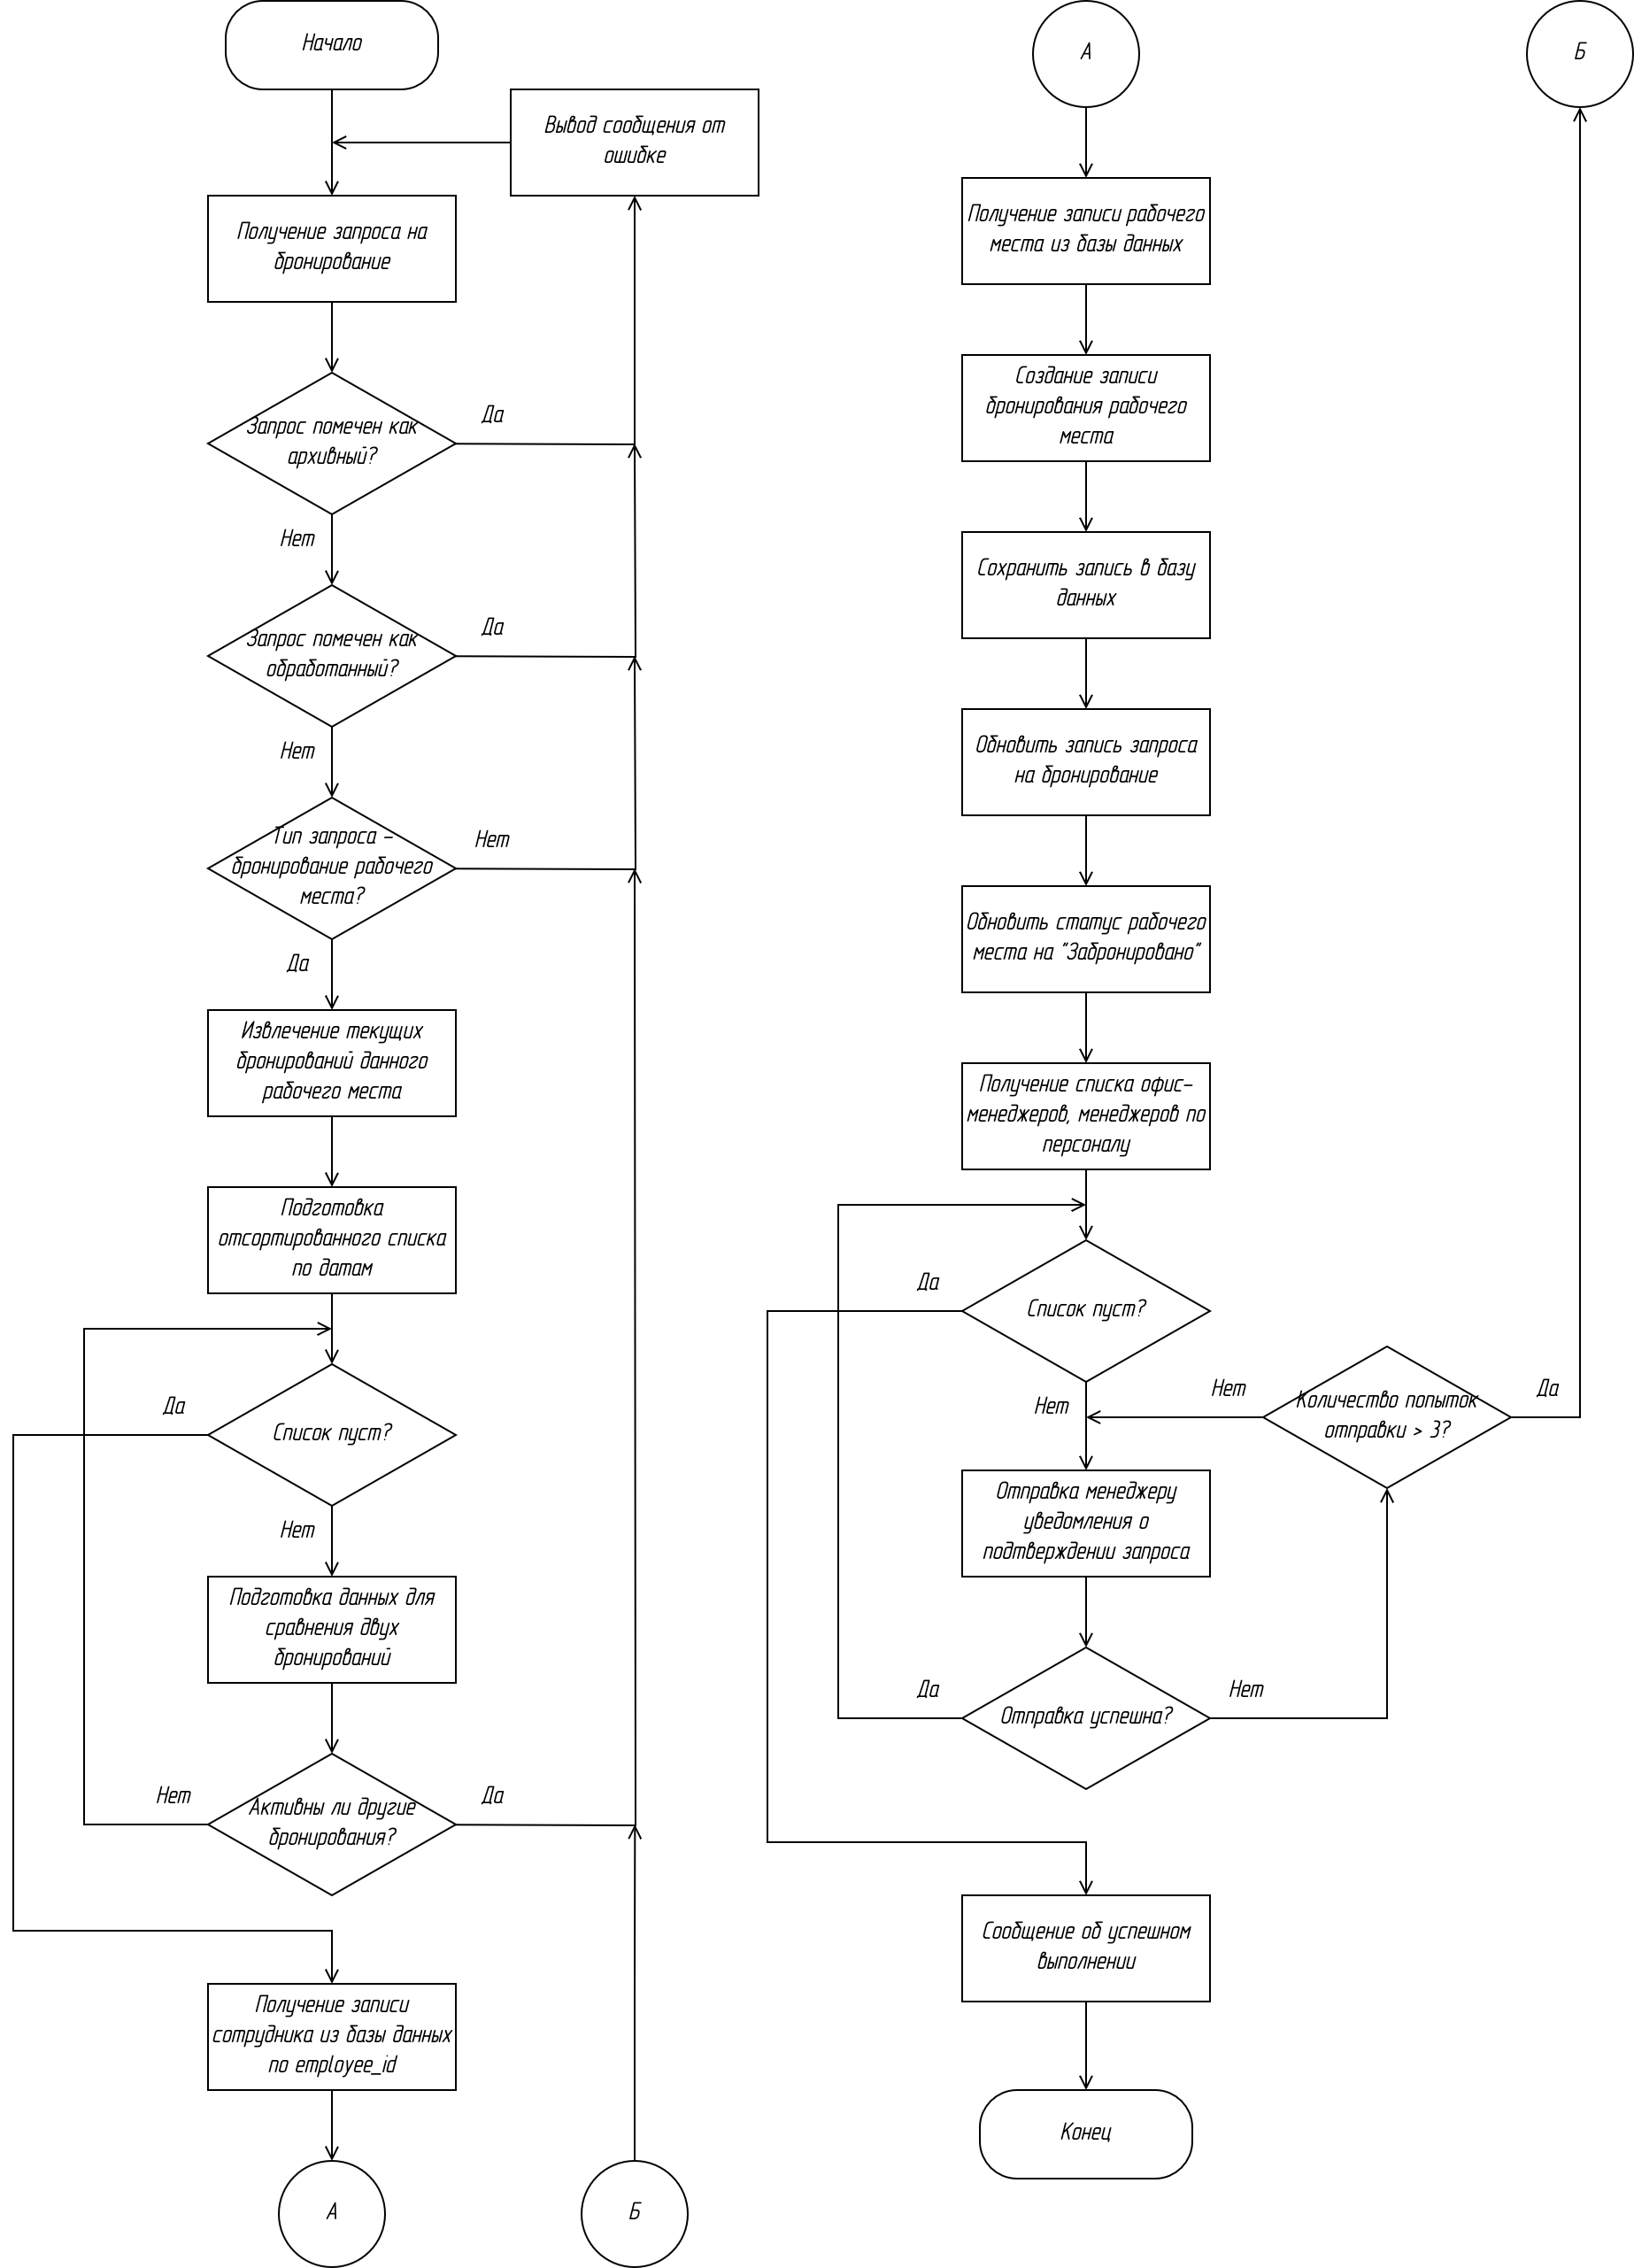
\includegraphics[width=0.99\linewidth]{assets/algorithm-approve-request.png}
    \caption{Схема алгоритма утверждения запроса на бронирование рабочего места}
    \label{fig:system-design:algorithms:approve-workspace-request}
\end{figure}

\textbf{Алгоритм автоматической рассадки сотрудников} предназначен для распределения сотрудников по рабочим местам в офисе на основе заранее заданных параметров. Основная цель~-- оптимально использовать офисные ресурсы, учитывать предпочтения сотрудников и ограничения, связанные с доступностью ресурсов, а также минимизировать ручной труд со стороны менеджеров.

Исходными данными к алгоритму будет являться список сотрудников, нуждающихся в рассадке на определённый период (например, дата или диапазон дат), список доступных рабочих мест, параметры предпочтений сотрудников, данные о занятости рабочих мест (бронирования, текущие рассадки, ремонт/неисправность и т.д.), правила рассадки (заданные компанией, например: сотрудники одного отдела~-- рядом, руководитель~-- возле окна и т.п.). Алгоритм содержит в себе несколько этапов проверки правильности входных значений и операций с базой данных.

\begin{enumerate}
    \item \textit{Получение списка сотрудников}, которые нуждаются в рассадке на определённую дату. В выборку включаются только активные сотрудники, у которых отсутствует назначенное рабочее место на этот день. Исключаются лица, находящиеся в отпуске, командировке, заблокированные или работающие удалённо.
    \item \textit{Определение доступных рабочих мест} путем извлечения из базы данных перечня рабочих мест, которые свободны в указанный период. При этом учитываются следующие ограничения:
    \begin{itemize}
        \item статус рабочего места (только «свободно»);
        \item отсутствие активных бронирований на соответствующий интервал;
        \item исправное техническое состояние;
        \item доступность в рамках политики доступа сотрудника (например, этаж, зона).
    \end{itemize}
    \item \textit{Построение матрицы предпочтений}. Для каждого сотрудника создаётся индивидуальный список предпочтительных рабочих мест, отсортированный по убыванию рейтинга соответствия. Рейтинг формируется на основе множества факторов:
    \begin{itemize}
        \item 3 балла~-- если место соответствует предпочтению «рядом с окном»;
        \item 2 балла~-- если этаж совпадает с желаемым;
        \item 2 балла~-- если место находится в тихой зоне, а сотрудник указал «тишина»;
        \item 2 балла~-- если рядом размещены коллеги из того же отдела;
        \item 1 балл~-- если место расположено вблизи полезной инфраструктуры (принтер, кухня, переговорная);
        \item 0 баллов~-- если критерий не соответствует или отсутствует.
    \end{itemize}
    Для каждого сотрудника инициализируется пустой список предпочтений, производится цикл по всем доступным рабочим местам, где вычисляется рейтинг для каждого места, вследствие чего формируется упорядоченный список подходящих мест. Данные сохраняются в общую матрицу предпочтений сотрудников.
    \item \textit{Проверка достаточности ресурсов}. Перед началом назначения производится проверка: достаточно ли свободных мест для всех сотрудников. Если количество сотрудников превышает число доступных мест, выполняется приоритизация (например, по должности или по срочности присутствия в офисе). Только первые \textit{N} сотрудников получают место, остальные же помечаются как «не рассажены» с соответствующей записью в журнале действий.
    \item \textit{Распределение сотрудников по местам}. Алгоритм последовательно обрабатывает каждого сотрудника, путем выполнения попыток назначить первое доступное место из списка предпочтений. При назначении создаётся запись рассадки, статус рабочего места меняется на «занято». Если ни одно из мест недоступно, сотрудник помечается как «нерассаженный» с указанием причины.
    \item \textit{Формирование отчёта}. По завершении рассадки система формирует отчёт, содержащий фамилию и имя сотрудника, назначенное рабочее место (офис, этаж, номер), степень соответствия предпочтениям, причину отсутствия места (если применимо). Отчёт сохраняется в виде внутреннего документа и может быть передан менеджеру или администратору для дальнейшего анализа.
    \item \textit{Уведомление участников}. На последнем этапе каждому сотруднику отправляется уведомление. В случае, если место назначено~-- сообщение с указанием конкретного места. Если рассадка не произведена~-- отправляется уведомление о необходимости обратиться к менеджеру. Уведомления могут доставляться через email, внутреннюю систему оповещений, или интеграцию с корпоративными мессенджерами.
\end{enumerate}

Результатом выполнения является достижение желаемого результата рассадки сотрудников, при котором каждому сотруднику назначено уникальное рабочее место с учетом предпочтений и ограничений, а также обновление статусов рабочих мест и создание записей о бронировании (рассадке). Алгоритм исключает конфликтные назначения, повышает прозрачность логики рассадки, обеспечивает контроль менеджеров и предоставляет полноценную отчётность по принятым решениям.

Схема алгоритма автоматической рассадки сотрудников представлена на рис.~\ref{fig:system-design:algorithms:automatic-workspace-occupation}.

\begin{figure}
\centering
    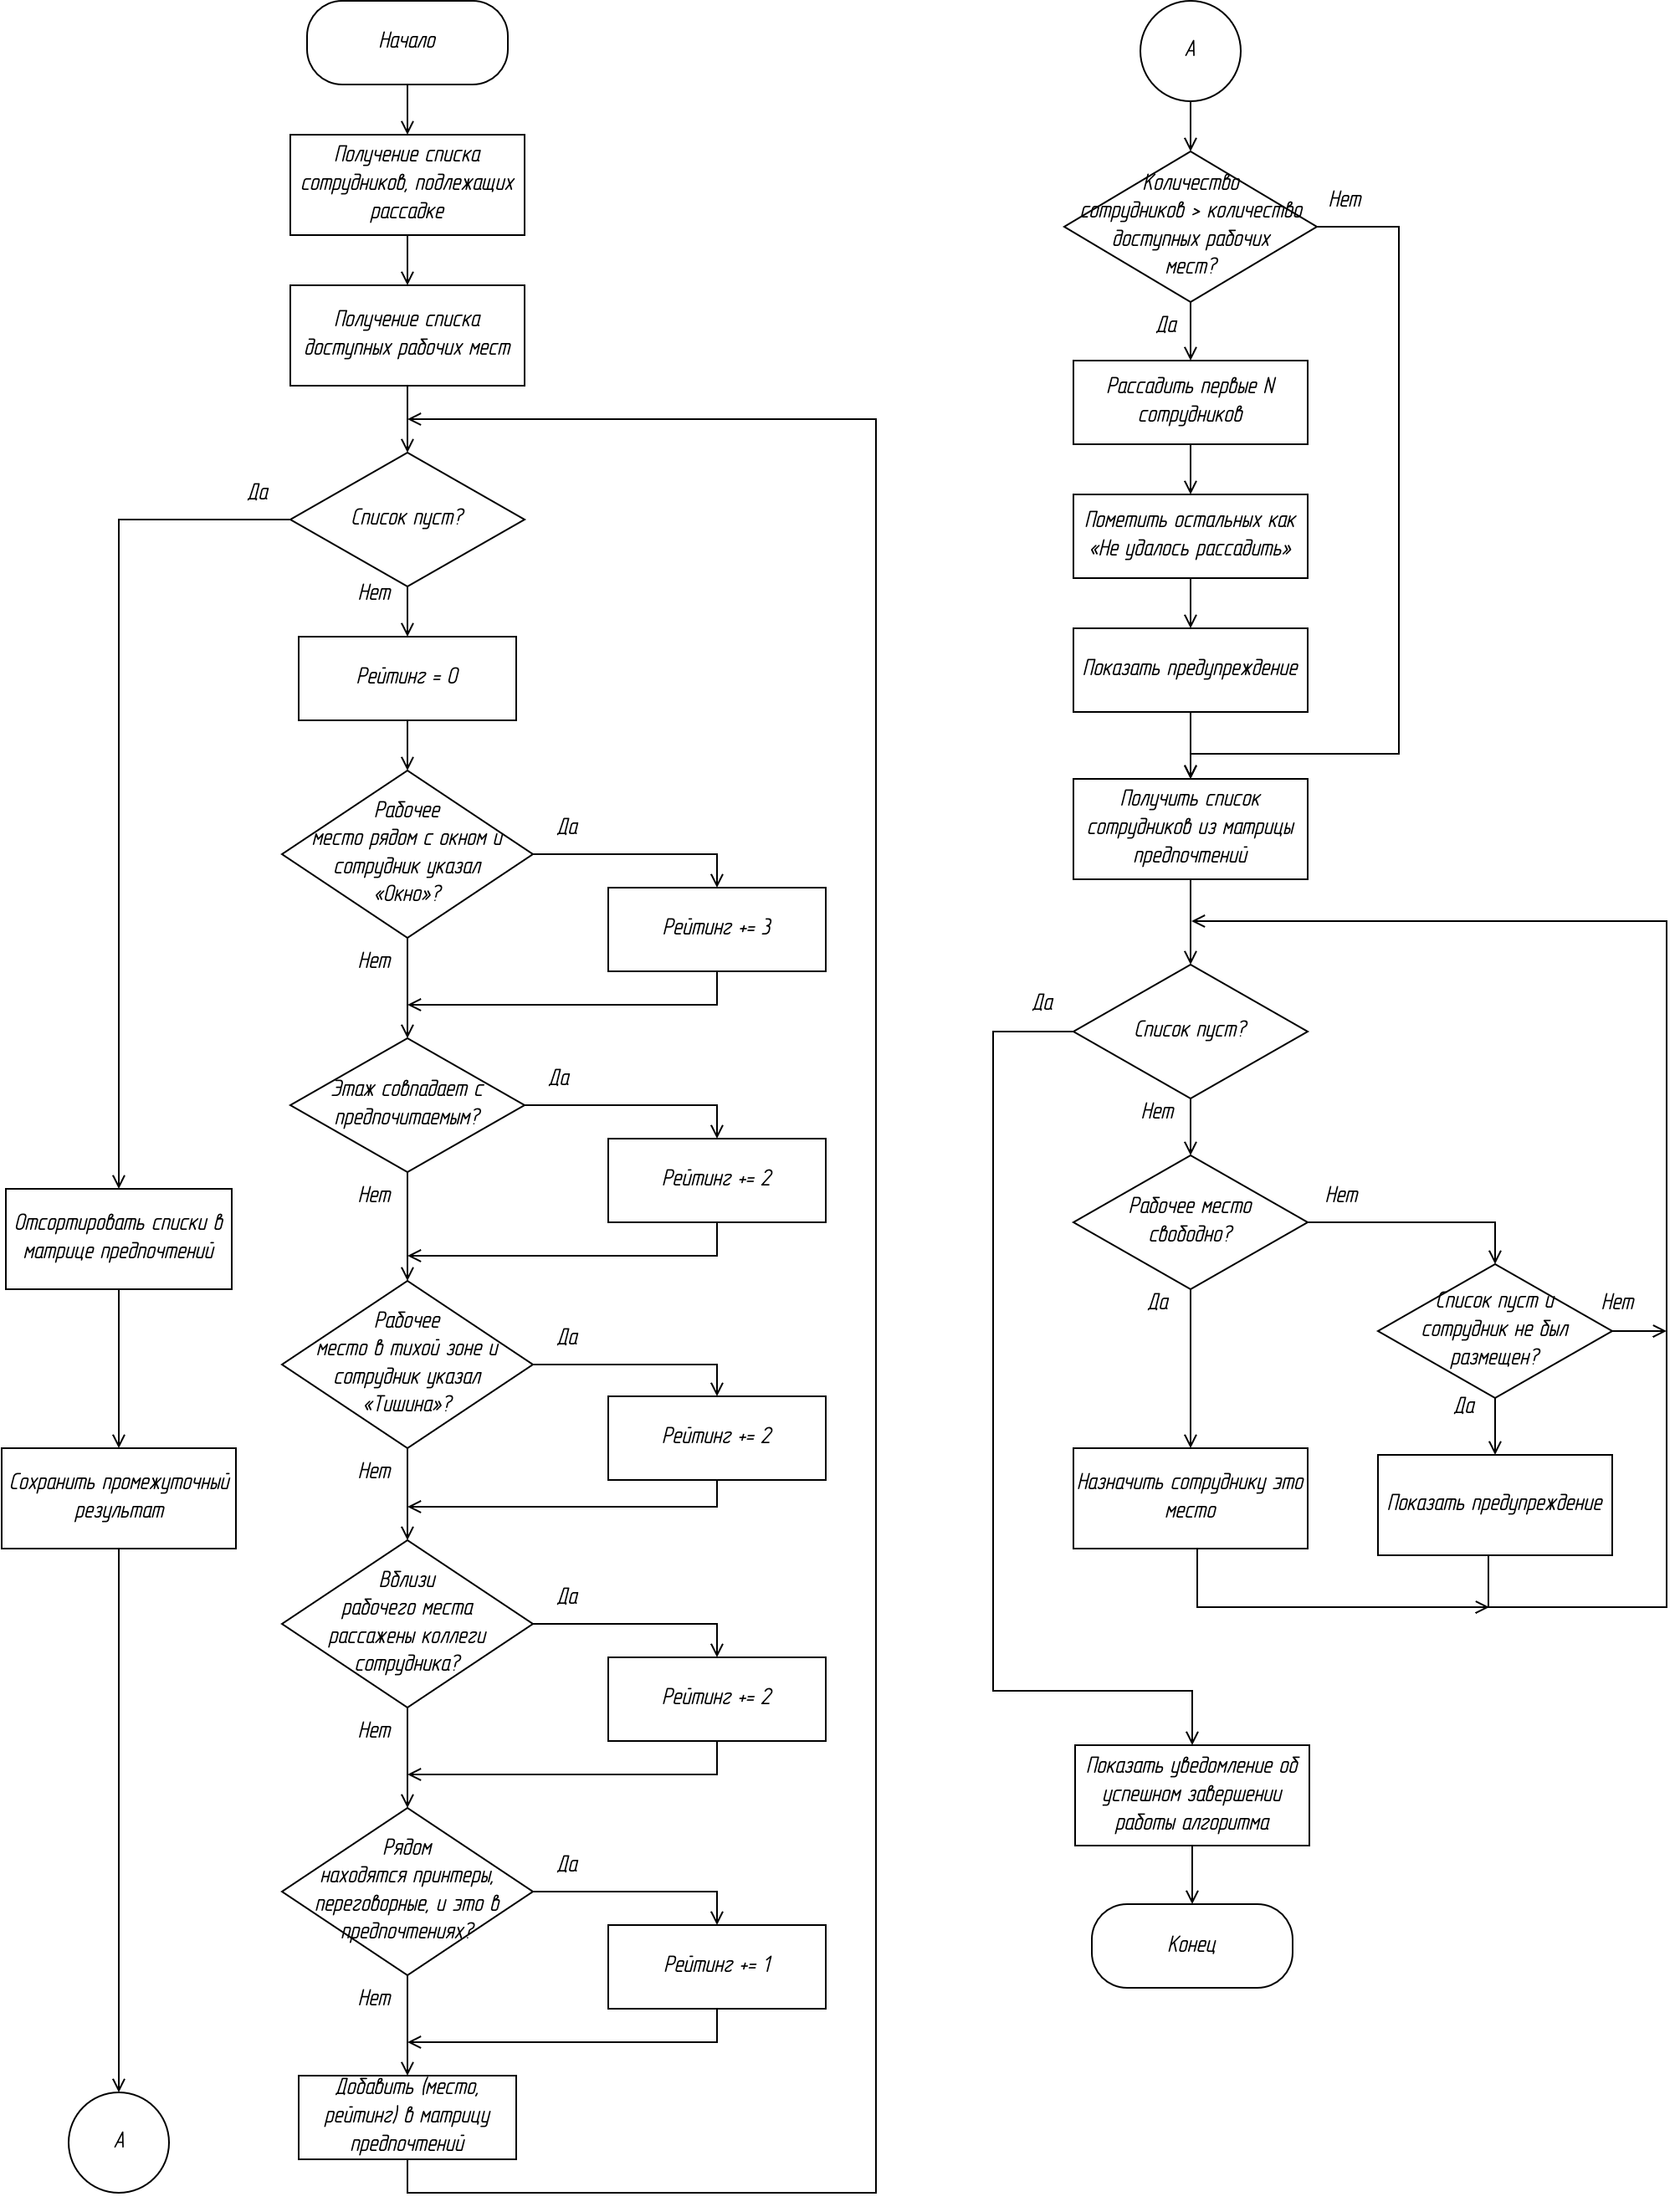
\includegraphics[width=0.99\linewidth]{assets/algorithm-automatic-workspace-occupation.png}
    \caption{Схема алгоритма автоматической рассадки сотрудников}
    \label{fig:system-design:algorithms:automatic-workspace-occupation}
\end{figure}


\subsection{Развёртывание модулей и сервисов системы}
\label{sub:system-design:deployment}

Развертывание~-- процесс, сочетающий две взаимосвязанные концепции~-- процесса и архитектуры. Процесс развертывания заключается в доставке кода в промышленную среду и состоит из этапов, которые должны выполнить разработчики или системные администраторы.

Облачные вычисления~-- это способ предоставления системных ресурсов компьютера по требованию без активного участия пользователя в их управлении. Частные случаи таких ресурсов~-- хранилище данных (облачное) и вычислительные мощности. Облачные вычисления предоставляются потребителям в разных формах. Моделей обслуживания всего три основных, хотя в рамках конкретных бизнес-потребностей модели могут принимать подвиды. На рис.~\ref{fig:cloud-computing-service-models} представлены основные сервисные модели облачных вычислений. Все эти модели являются слоями над физическими вычислительными ресурсами, так модель \textit{SaaS} включает в себя все слои ниже, с той лишь разницей что для клиентов облака остальные слои скрыты и взаимодействие с ними происходит только лишь через слой \textit{SaaS}.

\begin{figure}[h]
\centering
    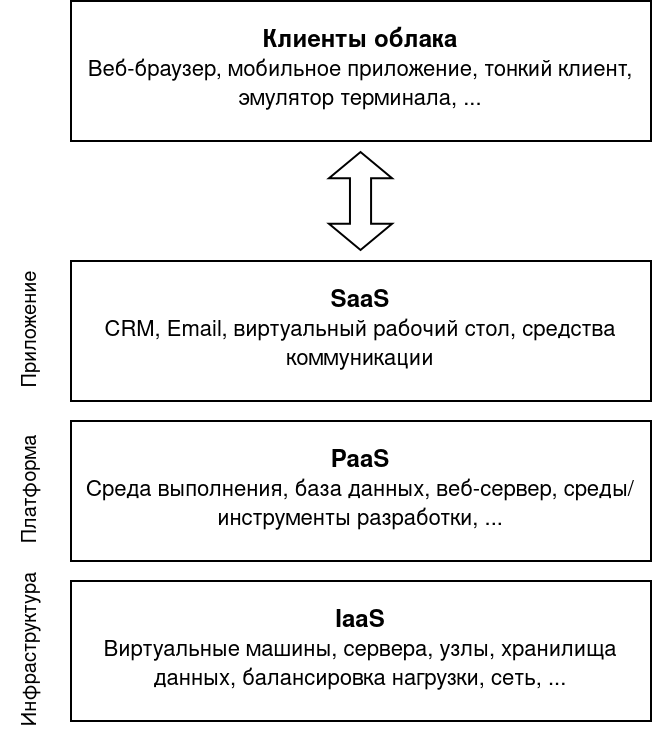
\includegraphics[width=0.5\linewidth]{assets/cloud-computing-service-models.png}
    \caption{Модели компьютерных вычислений в виде слоев}
    \label{fig:cloud-computing-service-models}
\end{figure}

\textit{Модель SaaS (Software as a Service)}~-- «Программное обеспечение как услуга»~-- модель, в которой потребителю предоставляется возможность использования прикладного программного обеспечения провайдера, работающего в облачной инфраструктуре и доступного из различных клиентских устройств или посредством клиента, например, из браузера (например, веб-почта) или посредством интерфейса программы.

\textit{Модель PaaS (Platform as a Service)}~-- «Платформа как услуга»~-- модель, когда потребителю предоставляется возможность использования облачной инфраструктуры для размещения базового программного обеспечения для последующего размещения на нём новых или существующих приложений (собственных, разработанных на заказ или приобретённых тиражируемых приложений). В состав таких платформ входят инструментальные средства создания, тестирования и выполнения прикладного программного обеспечения~-- системы управления базами данных, связующее программное обеспечение, среды исполнения языков программирования, предоставляемые облачным провайдером.

\textit{Модель IaaS (Infrastructure as a Service)}~-- «Инфраструктура как услуга» пре\-дос\-та\-вля\-ется как возможность использования облачной инфраструктуры для самостоятельного управления ресурсами обработки, хранения, сетями и другими фундаментальными вычислительными ресурсами, например, потребитель может устанавливать и запускать произвольное программное обеспечение, которое может включать в себя операционные системы, платформенное и прикладное программное обеспечение.

В рамках дипломного проекта в большей степени рассматривается модель \textit{PaaS}. Именно на этом слое разрабатываются микросервисы и формируется бизнес логика. Другими словами, именно на PaaS слое формируется слой выше (SaaS), который предоставляет уже конкретные услуги пользователям. Конкретными программными продуктами, реализующими модель PaaS, являются: \textit{Openshift}, \textit{Kubernetes}, \textit{Docker}, \textit{Docker Swarm}. Разработанный конечный продукт должен иметь возможность легко разворачиваться в любой из этих сред. Этого легко добиться, так как \textit{Openshift} платформа строится на \textit{Kubernetes}, а тот, в свою очередь, построен на основе \textit{Docker}. За счёт удачности решений эти программные продукты используются во многих компаниях и являются устоявшимся стандартом облачной разработки. Крупные провайдеры облачных платформ, такие как \textit{Amazon Web Services}, \textit{Google Cloud}, \textit{Microsoft Azure}, в том числе белорусский \textit{Hoster.by}, предоставляют возможность развернуть любой из приведенных выше продуктов.

С разработкой программного продукта необходимо разработать и схему процесса его автоматизированного развертывания в облаке, потому что конфигурация развертывания должна быть опубликована в \textit{PaaS}, чтобы процесс жизненного цикла приложения начался. Одной из особенностей облачных окружений является файл конфигурации развертывания~-- \textit{Deployment}, который непосредственно публикуется в среде \textit{PaaS}. В рамках дипломного проекта рассматривается \textit{PaaS} среда \textit{Kubernetes}~-- инструмент оркестрации \textit{Docker}, который обращается с набором серверов под управлением \textit{Docker}, как с пулом ресурсов. Архитектура фреймворка оркестрации \textit{Docker} представлена на рис.~\ref{fig:system-design:deployment:kubernetes-infrastructure}.

\begin{figure}[h]
\centering
    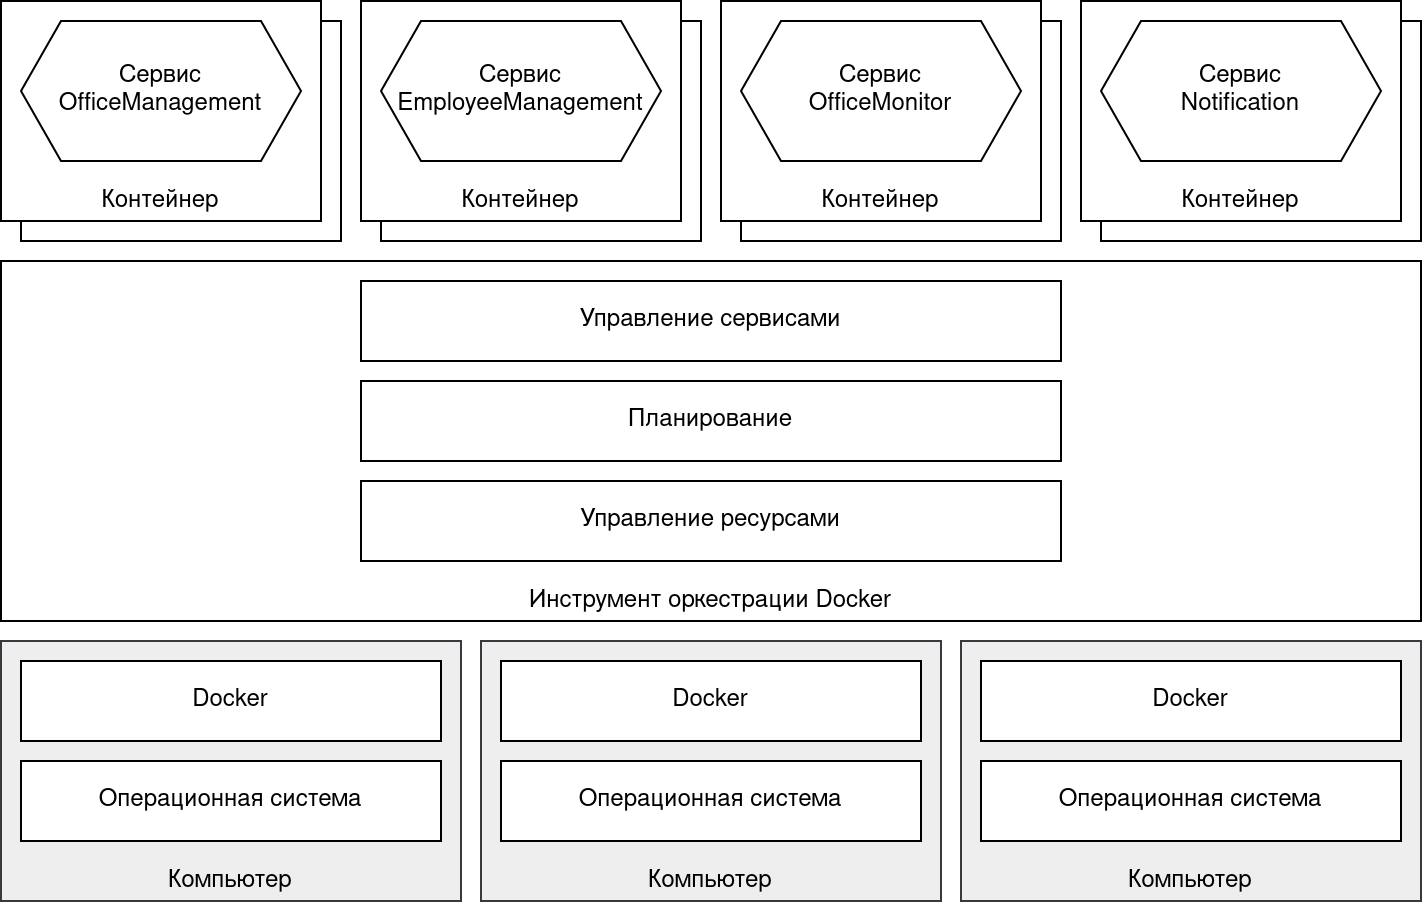
\includegraphics[width=0.99\linewidth]{assets/kubernetes-infrastructure.png}
    \caption{Архитектура \textit{Kubernetes}}
    \label{fig:system-design:deployment:kubernetes-infrastructure}
\end{figure}

Листинг конфигурации \textit{Deployment} \textit{Kubernetes} для развертывания микросервиса \textit{EmployeeManagement} приведен ниже:

\begin{lstlisting}[style=pythonstyle]
apiVersion: apps/v1
kind: Deployment
metadata:
  name: employee_management_service-backend-deployment
  namespace: office_management-production
spec:
  replicas: 2
  selector:
    matchLabels:
      type: backend
      service: employee_management
  strategy:
    type: RollingUpdate
    rollingUpdate:
      maxSurge: 1
      maxUnavailable: 1
  minReadySeconds: 10
  template:
    metadata:
      labels:
        type: backend
        service: employee_management
    spec:
      initContainers:
        - name: migrate
          image: employee_management_service-backend:latest
          envFrom:
            - secretRef:
                name: employee_management_service-backend-secrets
      containers:
        - name: backend
          image: employee_management_service-backend:latest
          envFrom:
            - secretRef:
                name: employee_management_service-backend-secrets
          ports:
            - containerPort: 8001
          resources:
            requests:
              memory: "512Mi"
              cpu: "250m"
            limits:
              memory: "1024Mi"
              cpu: "500m"
          readinessProbe:
            httpGet:
              path: /api/healthcheck
              port: 8001
            initialDelaySeconds: 10
          livenessProbe:
            httpGet:
              path: /api/healthcheck
              port: 8001
            initialDelaySeconds: 10
\end{lstlisting}

Важным пунктом конфигурации является свойство \textit{\lstinline!image!}, в нем указано имя образа контейнера, который будет браться из настроенного на хост машине репозитория \textit{Docker}-образов. Для большей наглядности изобразим полный путь контейнера от момента его создания (сборки) до момента попадания на хост машину с \textit{Kubernetes}. Свой жизненный путь \textit{Docker}-образ берет с исходного кода и \textit{Dockerfile}, где описано из чего создается образ, какие файлы, инструменты и программы он содержит в себе. Диаграмма состояния процесса сборки исходного кода микросервиса в \textit{Docker}-образ изображена на рис.~\ref{fig:docker-image-flow}.

\begin{figure}[h]
\centering
    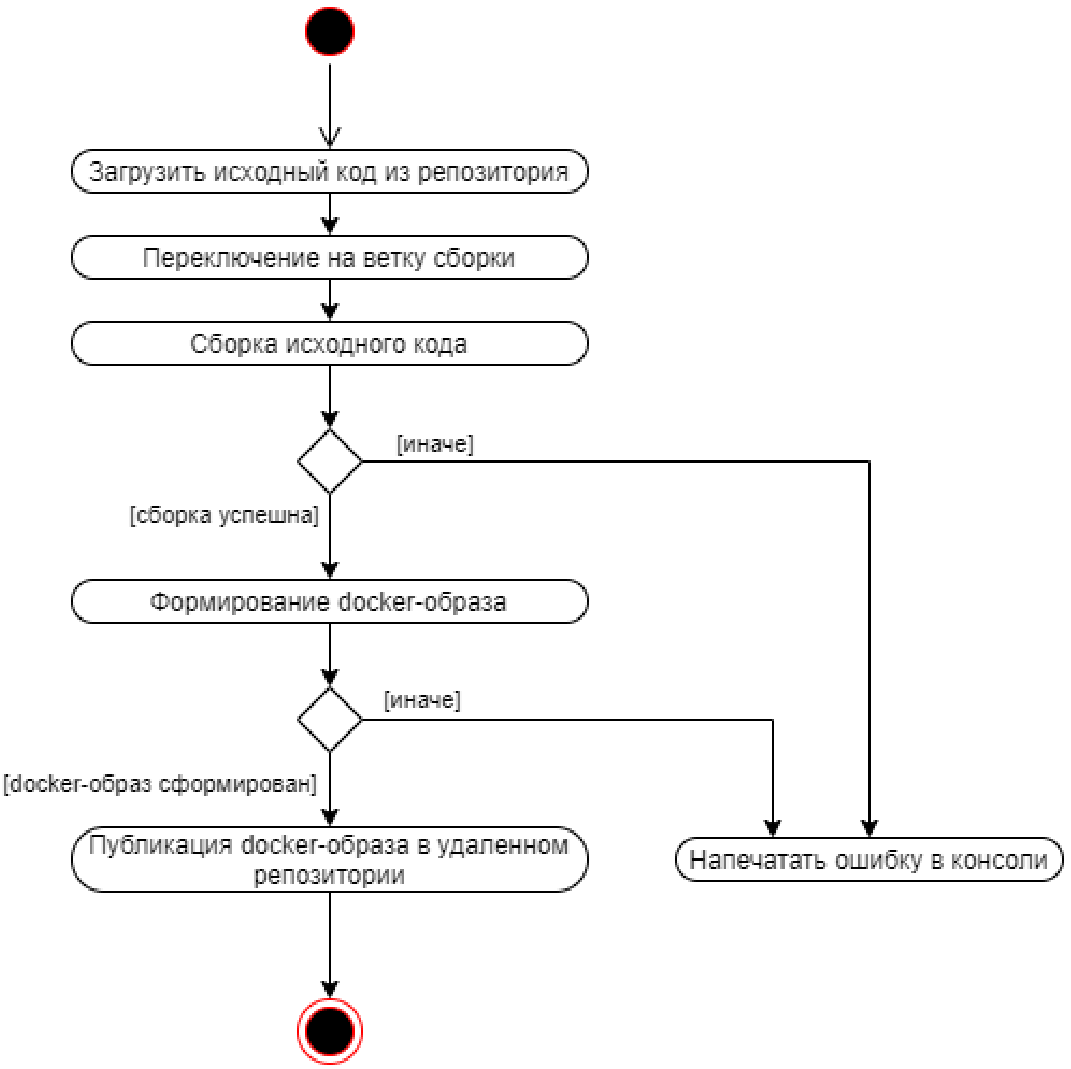
\includegraphics[width=0.75\linewidth]{assets/docker-image-flow.png}
    \caption{Диаграмма состояния процесса сборки исходного кода микросервиса в \textit{Docker}-образ}
    \label{fig:docker-image-flow}
\end{figure}

Рассмотрим концептуальную схему работы программного средства. Клиенты взаимодействуют с сервисами, предназначенными для сокрытия набора \textit{Pod} под одним \textit{DNS} именем. Например, возможен вариант реализации нескольких экземпляров \textit{API-Gateway} запущенных в облаке, однако обращение к ним возможно через \textit{DNS} имя \textit{\lstinline!api-gateway!}. Таким образом, \textit{Service} в \textit{Kubernetes}~-- это \textit{DNS} запись, скрывающая несколько \textit{IP}-адресов запущенных экземпляров приложения~\cite{book_production_kubernetes}. Набор \textit{Pod}-экземпляров является олицетворением запущенных \textit{Docker} контейнеров. Жизненный цикл \textit{Pod} определяется ресурсом \textit{Deployment}, рассмотренным ранее. Фигурой документа изображены самописные ресурсы, опубликованные в облаке, которые создаются и описываются разработчиком.

Под клиентом подразумевается либо человек, либо другой микросервис, который использует опубликованное \textit{API}. Взаимодействие с сервисами выражено путем отправки \textit{HTTP}-запросов к \textit{API-Gateway}, который при наличии соответствующего правила маршрутизации перенаправит запрос к целевому микросервису. На рисунке~\ref{fig:kubernetes-conceptual-architecture} представлена облачная среда под управлением \textit{PaaS} \textit{Kubernetes}. Все фигуры, кроме клиентов обозначают серверные облачные ресурсы. 

\begin{figure}[h]
\centering
    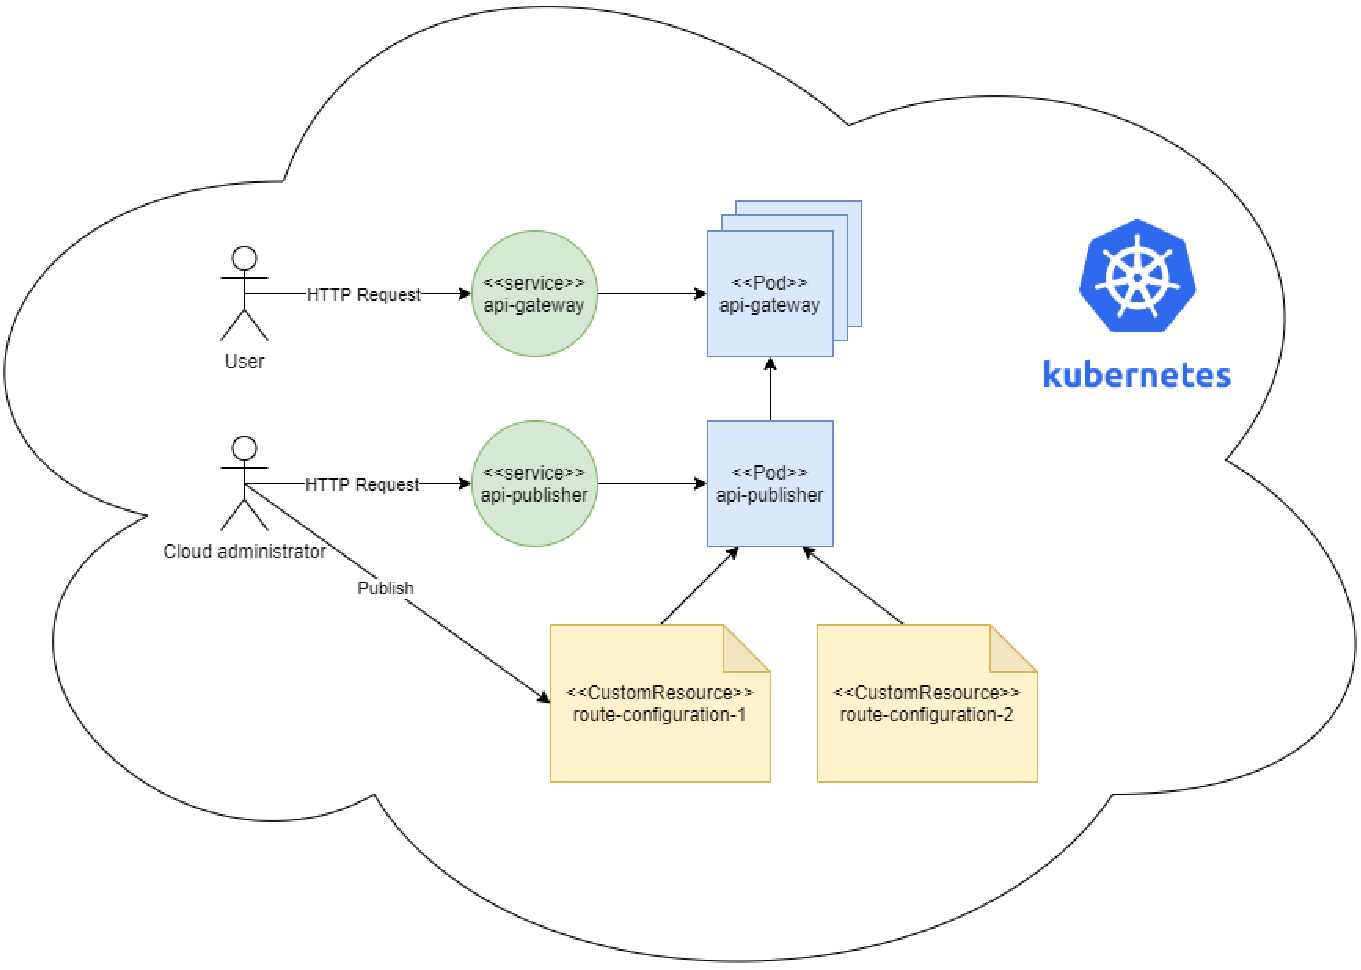
\includegraphics[width=0.8\linewidth]{assets/kubernetes-conceptual-architecture.png}
    \caption{Концептуальная архитектура \textit{PaaS} \textit{Kubernetes}}
    \label{fig:kubernetes-conceptual-architecture}
\end{figure}



В результате проектирования системы реализована гибридная архитектура, сочетающая клиент-серверную модель с микросервисным подходом. Серверная часть представлена автономными микросервисами: \textit{Employee\-Ma\-na\-ge\-ment}, \textit{OfficeManagement}, \textit{OfficeMonitor}, \textit{Notification}; каждый из которых инкапсулирует специфическую бизнес-логику, имеет собственную базу данных и взаимодействует с другими сервисами через брокер асинхронных сообщений, что повысило отказоустойчивость и упростило эволюцию системы. Для реализации выбраны \textit{Python} с \textit{FastAPI}, \textit{TypeScript} и \textit{React}, \textit{PostgreSQL} и \textit{Docker/Kubernetes}. База данных построена на реляционной модели с изолированными схемами для микросервисов. Развертывание ориентировано на \textit{Kubernetes} в модели PaaS, обеспечивающий оркестрацию, балансировку нагрузки и отказоустойчивость. 

Итогом проектирования стала модульная, масштабируемая система, соответствующая современным требованиям. Комбинация микросервисной архитектуры, серверных технологий и автоматизированных процессов разработки обеспечивает адаптивность к изменениям бизнес-требований, высокую доступность и безопасность данных, а также эффективное использование ресурсов.
